\documentclass[Nike]{tuberlinbeamer}

\usepackage{dsfont}

%\usepackage[ngerman]{babel}  % 'babel' muss geladen werden
\usepackage[utf8]{inputenc}  % optional, aber empfehlenswert
\usepackage[square,numbers]{natbib}
\usepackage{bibentry}




\usepackage[]{algorithm2e}
\usepackage{caption}
\captionsetup[figure]{labelformat=empty}
\usepackage[ddmmyyyy]{datetime}
\usepackage{subcaption}



% Die ueblichen Angaben
\title{Designing Recurrent Neural Networks for Explainability}
\subtitle{\today}
\author[TU Berlin]{Pattarawat Chormai}
\institute{Technische Universität Berlin}

% Eigenes Logo einfuegen:
\renewcommand{\pathtomylogo}{}
\newcommand{\x}[0]{\boldsymbol{x}}
\newcommand{\pvec}[1]{\boldsymbol{#1}}
\newcommand{\ppartial}[2]{\frac{\partial #1}{\partial #2}}
\renewcommand{\pagename}{Page} 



\begin{document}

\begin{frame}
\maketitle
\end{frame}


%\begin{frame}{Outline}
%\tableofcontents
%\end{frame}


%\section{Objective}	
\begin{frame}{Motivation}

\begin{itemize}
	\item Impact of the architecture of RNNs on explainability
	\item Are deep RNNs more explainable? 
	\item Are there ways to make RNNs more explainable?
\end{itemize}
\end{frame}

\begin{frame}{Recurrent Neural Networks (RNNs)}

\only<1>{
	\begin{figure}[h]
		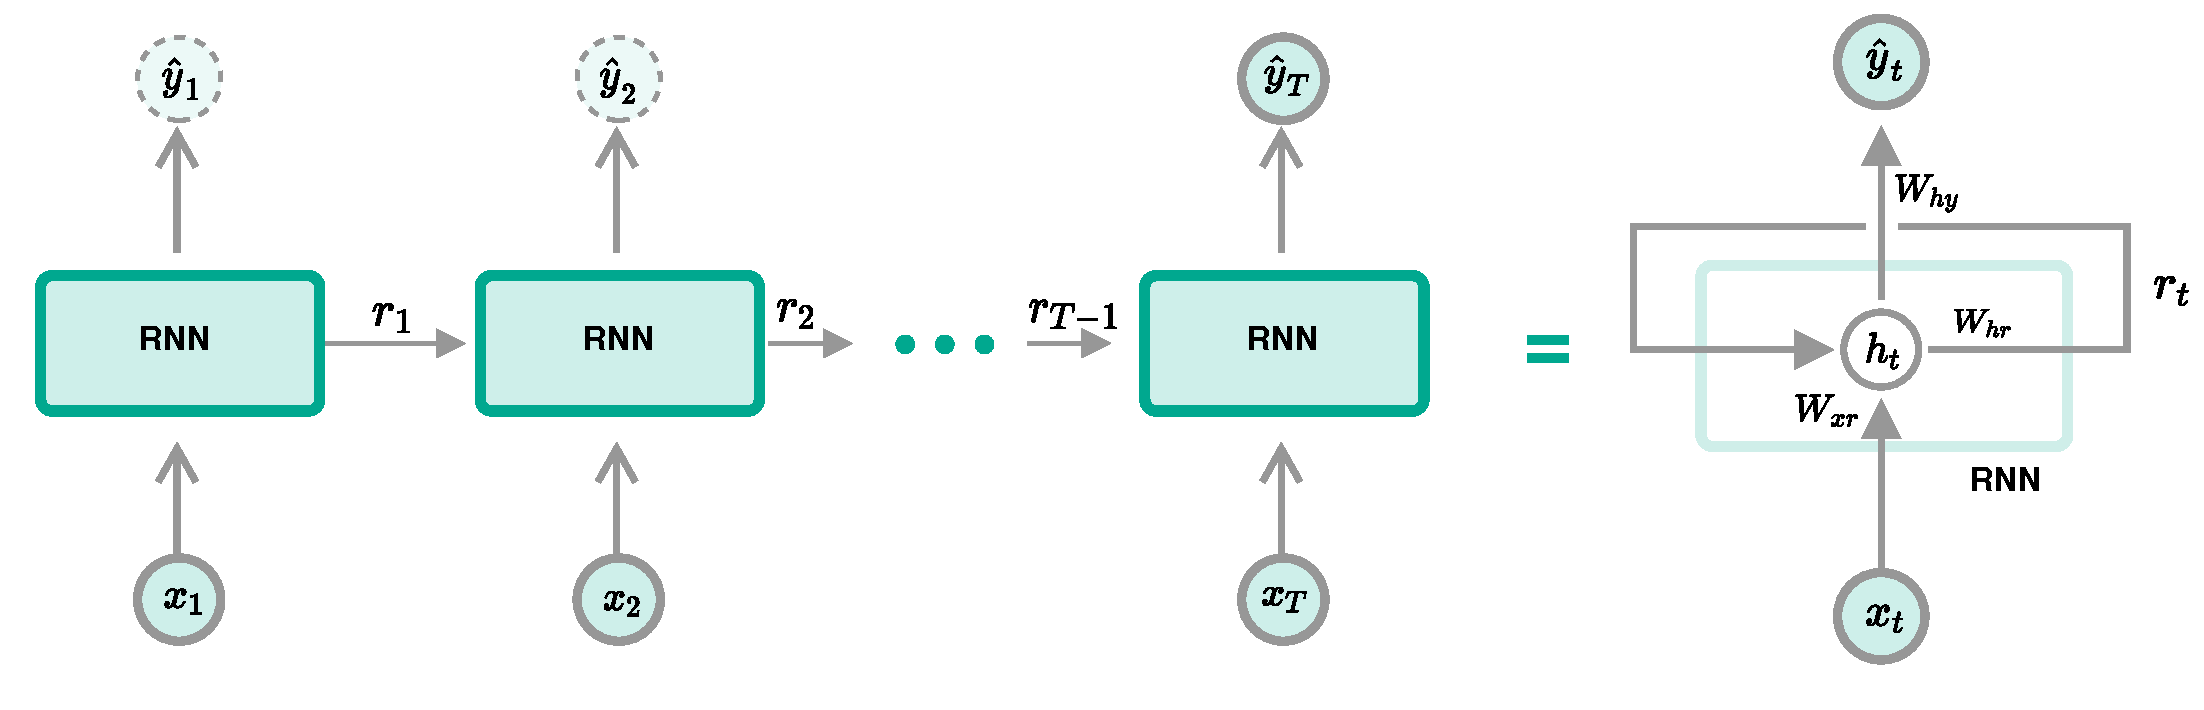
\includegraphics [width=\textwidth]{figures/present_rnn_unfold_1}
	\end{figure}
}

%\only<2>{
%	\begin{figure}[h]
%		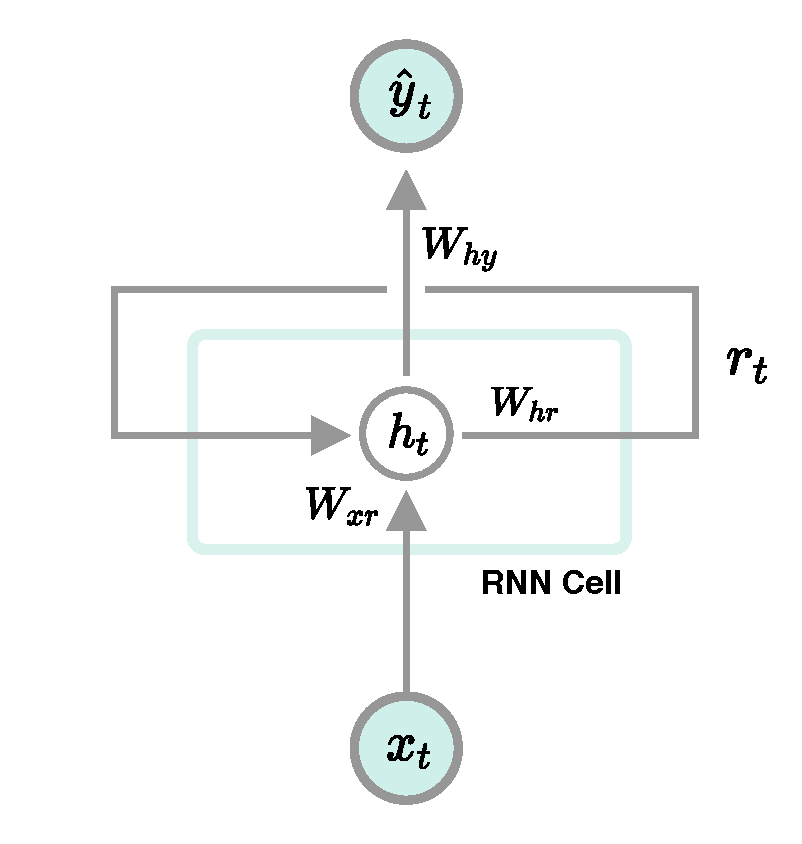
\includegraphics [width=0.4\textwidth]{figures/present_rnn_unfold_2}
%	\end{figure}
%}

\only<2>{
	\begin{itemize}
		\item Applications: sentiment analysis, NLP, machine translation, and image captioning
	\end{itemize}
	\begin{figure}[h]
		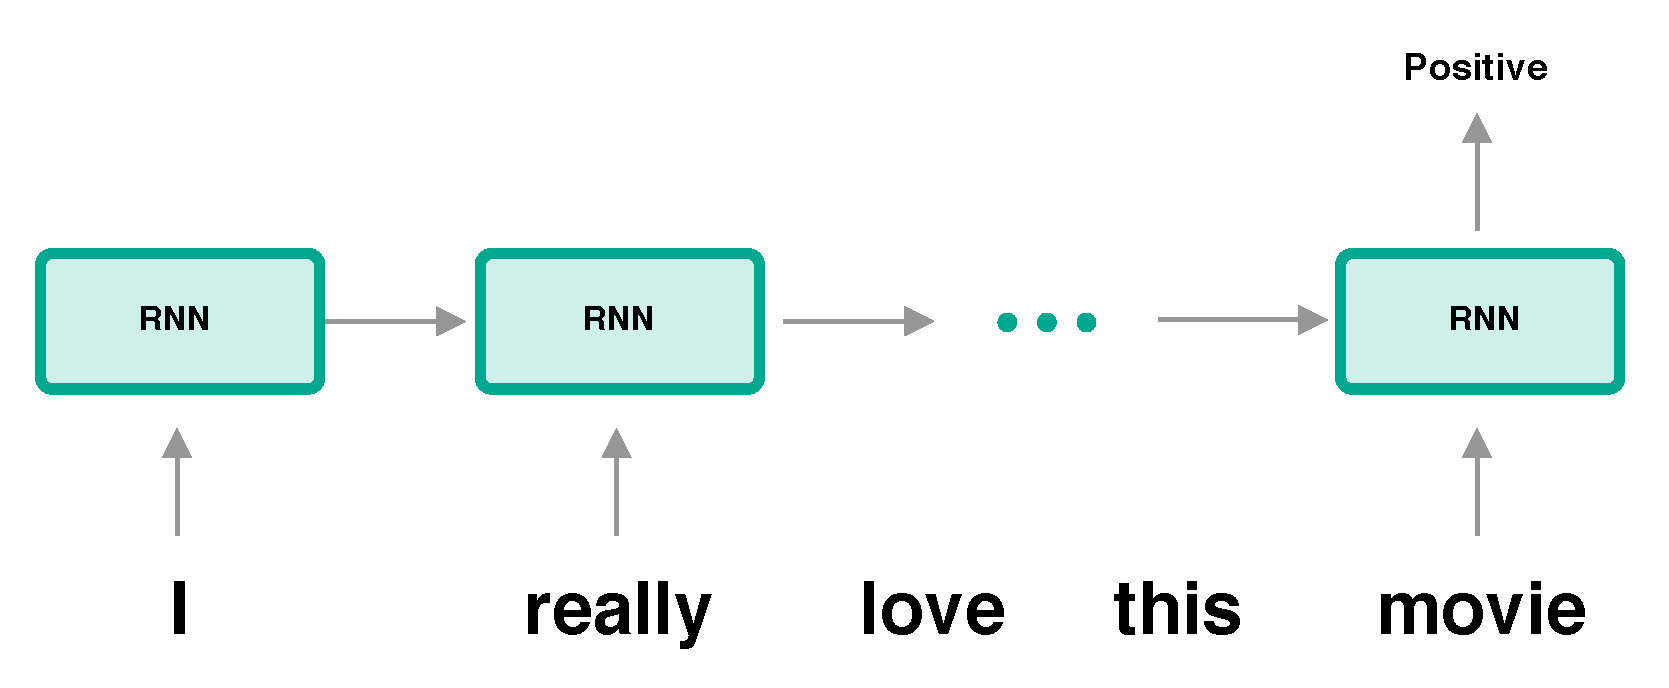
\includegraphics [width=0.8\textwidth]{figures/present_rnn_unfold}
	\end{figure}
}
%\only<3->{
%	\begin{itemize}
%		\item Typical neural networks have \textbf{a couple of millions} learnable parameters.
%	\end{itemize}
%}
 	
\end{frame}

\begin{frame}{Explainability}
\begin{itemize}
	\item Ability to provide sensible explanation towards how input associates to a particular output.
	\item For example, why does the RNN classify this text as a positive review?

	\begin{figure}[h]
		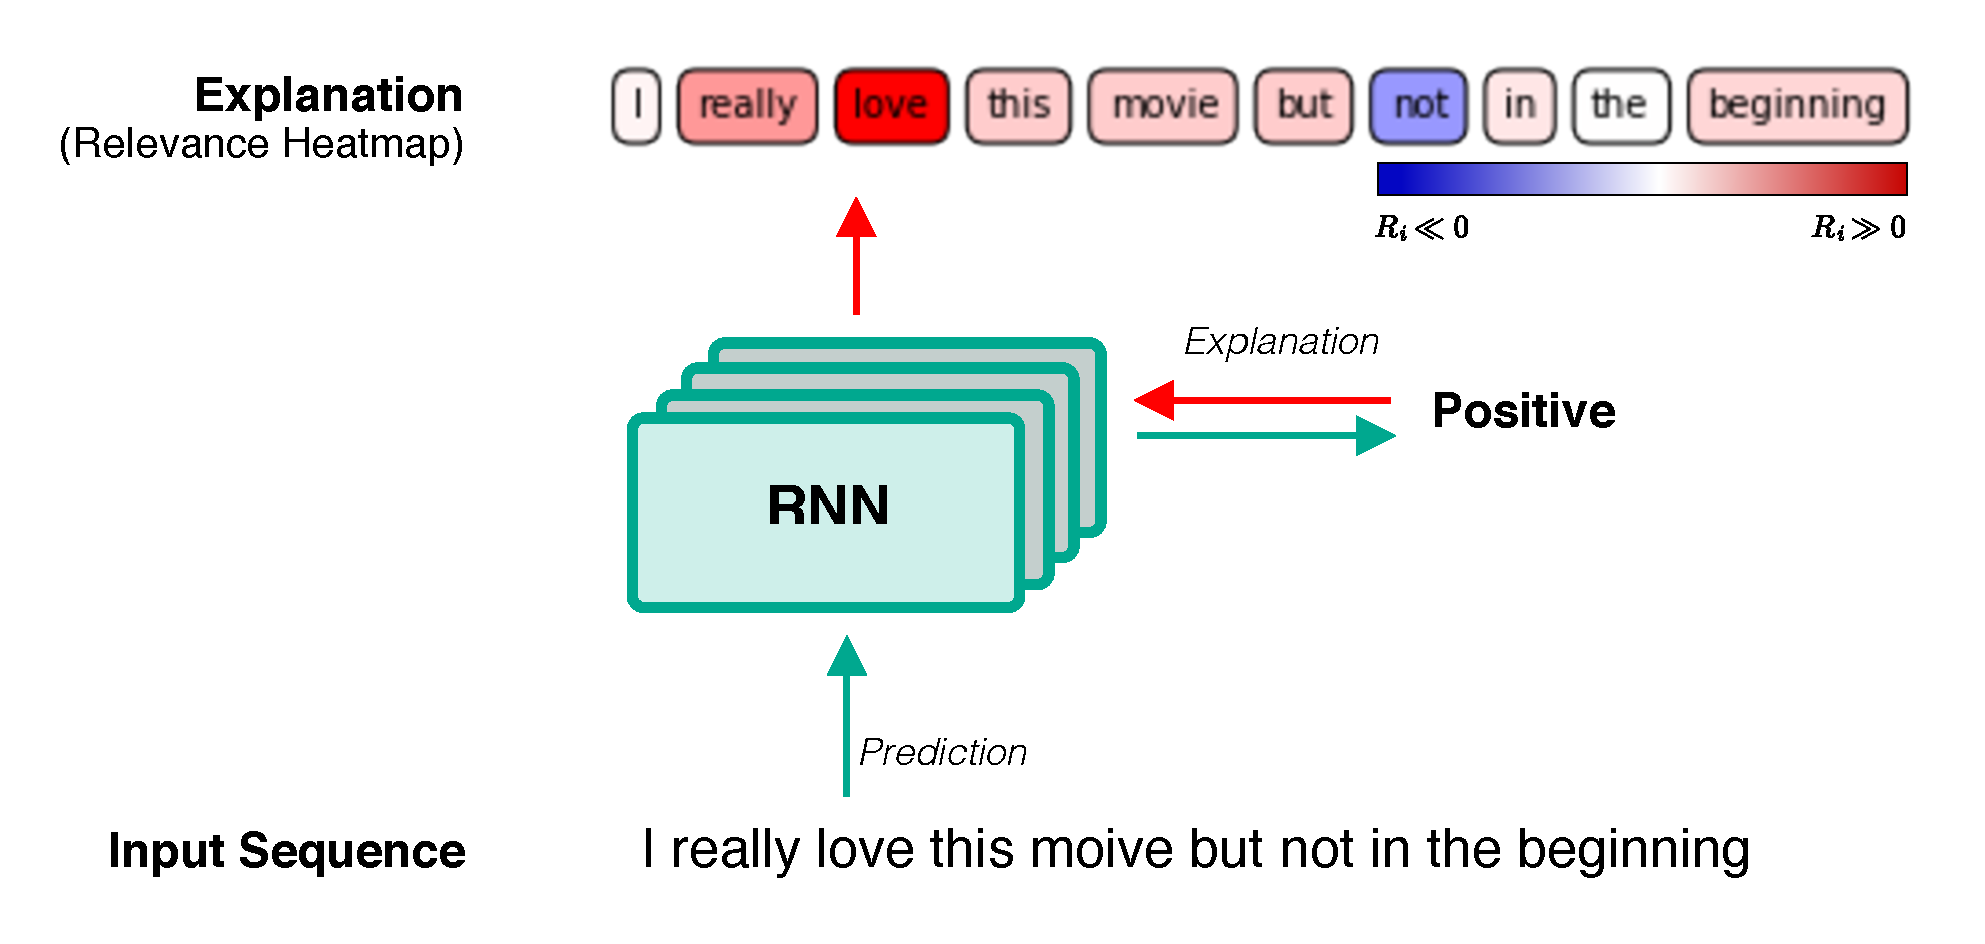
\includegraphics [width=0.65\textwidth]{figures/present_explanation_rnn}
	\end{figure}
	
%	\item Why do we need explainable models?\begin{itemize}
%		\item Aid decision and establish trust in the system, especially in critical applications such as healthcare.
%	\begin{figure}[h]
%		\centering
%%		\begin{subfigure}[b]{0.45\linewidth}
%%		  \centering
%%
%%			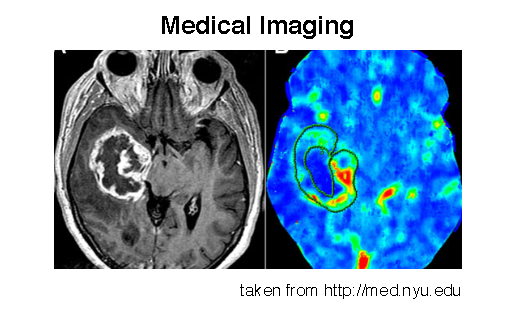
\includegraphics [width=0.9\textwidth]{figures/present_medical_imaging_cnn}
%%		\end{subfigure}
%		\begin{subfigure}[b]{0.5\linewidth}
%		  \centering
%
%			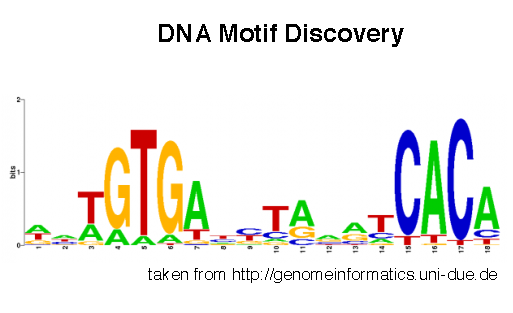
\includegraphics [width=0.9\textwidth]{figures/present_motif_discovery}
%		\end{subfigure}
%	\end{figure}
%		\item Developers can assure that trained models would work as expected.
%		\end{itemize}
\end{itemize}
	
\end{frame}



\section{Explanation Methods}
\begin{frame}[allowframebreaks=0.95,t]{Explanation Methods}

\begin{enumerate}
	\item Sensitivity Analysis \citep{SimonyanDeepConvolutionalNetworks2013}
			\begin{align*}
				R_i(\x) = \bigg ( \ppartial{f(\x)}{x_i} \bigg )^2
			\end{align*}
	\item Guided Backprop \citep{SpringenbergStrivingSimplicityAll2015a} \\
		\begin{itemize}
			\item Developed for explaining \textbf{ReLU}-based CNNs
		\end{itemize}
				\begin{align*}
				\frac{\partial_{*} f(\x) }{\partial h_j} = \mathds{1} \bigg[  h_j > 0 \bigg]\max\bigg( 0, \frac{\partial_{*} f(\x) }{\partial a_j} \bigg);\hspace{1cm} R_i(\x) = \bigg( \frac{\partial_{*} f(\x) }{\partial x_i} \bigg )^2
%				R_i(\x) = \bigg ( \frac{\partial #1}{\partial #2}\ppartial{f(\x)}{\x} \bigg )^2
			\end{align*}
	\framebreak
	
	\item Layer-wise Relevance Propagation (LRP) \citep{BinderLayerWiseRelevancePropagation2016} 
		\begin{itemize}
			\item Distributing relevance based on neurons' activities
			\begin{columns}
			\column{0.5\textwidth}{
				\begin{figure}[h]
					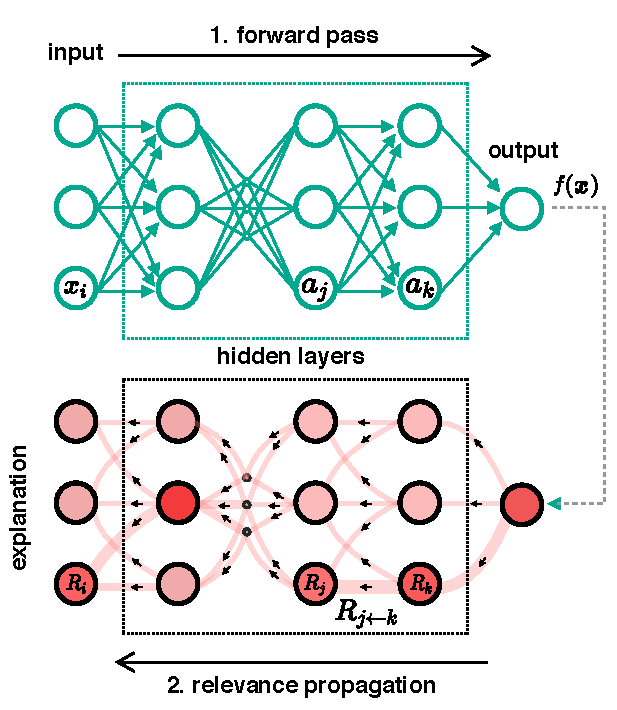
\includegraphics [width=0.75\textwidth]{figures/present_lrp_graph}
				\end{figure}

			}
			\column{0.5\textwidth}{
			   \vspace{1.5cm}\\
			LRP-$\alpha\beta$ rule:
			\begin{align*}
				R_j(\x) = \sum_k \bigg( \alpha \frac{a_j w_{jk}^+}{\sum_{j'} a_{j'} w_{j'k}^+}  - \beta  \frac{a_j w_{jk}^-}{\sum_{j'} a_{j'} w_{j'k}^-}  \bigg) R_k(\x)
			\end{align*}
			}
		\end{columns}

		\end{itemize}
	\vspace{3cm}
	
	 \item Deep Taylor Decomposition  \citep{MontavonExplainingnonlinearclassification2017}
		\begin{itemize}
			\item LRP's theoretical view for explaining \textbf{ReLU-based} architectures
			\begin{align*}
				R_k = R_k \bigg|_{\{ \tilde{a}_j \}_j} + \sum_j \frac{\partial R_k}{\partial a_j} \bigg|_{\{ \tilde{a}_j \}_j} (a_j - \tilde{a}_j ) + \xi_k \tag{Taylor expansion}
			\end{align*}
			\item Two important propagation rules:  \\
			-- $z^+$ for $a_j \in \mathbb{R}^+$ (LRP-${\alpha_{1}\beta_{0}}$)
			\begin{align*} 
				R_j  = \sum_k \frac{a_j w_{jk}^+ }{\sum_j a_j w_{jk}^+ }R_k 
			\end{align*}
			-- $z^\mathcal{B}$ for $a_j \in [l_j, h_j]$ where $l_j \le 0 < h_j$
			\begin{align*}
								R_j = \sum_k \frac{a_j w_{jk} - l_j w_{jk}^+ - h_j w_{jk}^- }{\sum_{j'} a_{j'} w_{j'k} - l_{j'} w_{j'k}^+ - h_{j'} w_{j'k}^- } R_k
			\end{align*}
		\end{itemize}
\end{enumerate}	
\end{frame}

%\begin{frame}{Example of relevance heatmaps}
%-- Explaining the classification decisions of a LeNet-5 type network.
%				\begin{figure}[h]
%					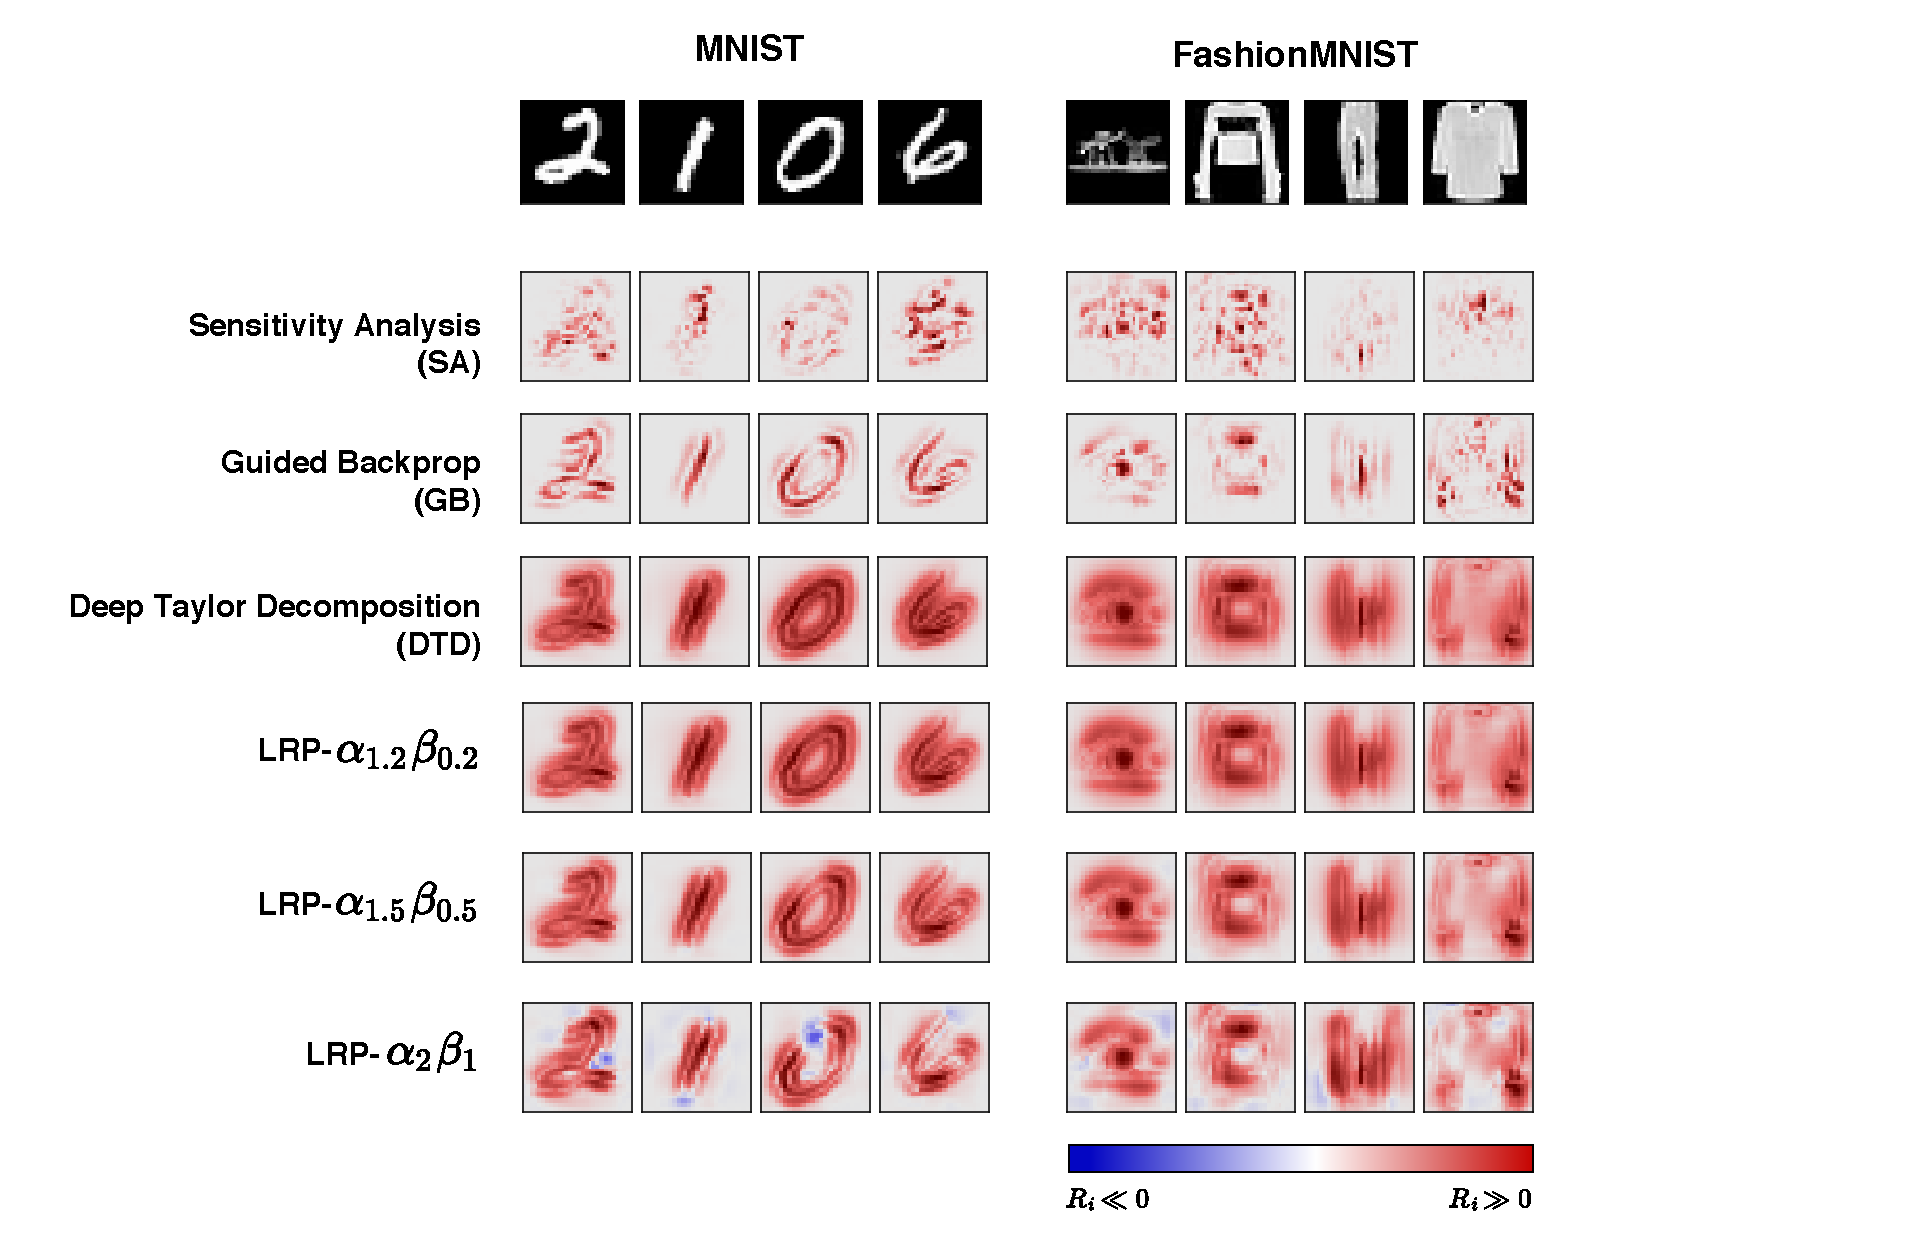
\includegraphics [width=0.7\textwidth]{figures/present_lenet_heatmaps}
%					\caption{ \tiny
%					Architecture: 
%								CONV(5$\times$5, 10) $\cdot$ AVGPOOL(2$\times$2, 2, 2) $\cdot$ 
%								CONV(5$\times$5, 25) $\cdot$ 
%								AVGPOOL(2$\times$2, 2, 2) $\cdot$
%								CONV(4$\times$4, 100)$\cdot$
%								AVGPOOL(2$\times$2, 2, 2) $\cdot$
%								DENSE(100) $\cdot$ DENSE(10)
%					}
%				\end{figure}
%
%%	 -  -  - AVG_POOL(2x2, 2, 2) - CONV(4x4, 100) - AVG_POOL(2x2, 2, 2)  - Dense(100) - DENSE (10)
%\end{frame}

\begin{frame}{Experimental Setup}
\begin{itemize}
	\item <1-3> \textbf{Problem:} Majority-Sample Sequence Classification
\only<1>{
	\newline
	$\rhd$ Minimum accuracy 98\% for MNIST and 89\% for FashionMNIST \\
	$\rhd$ Sequence length: 12 \big($\{\x_t \in \mathbb{R}^{28\times7} \}_{t=1}^{12}$ \big)

 \begin{figure}[h]
	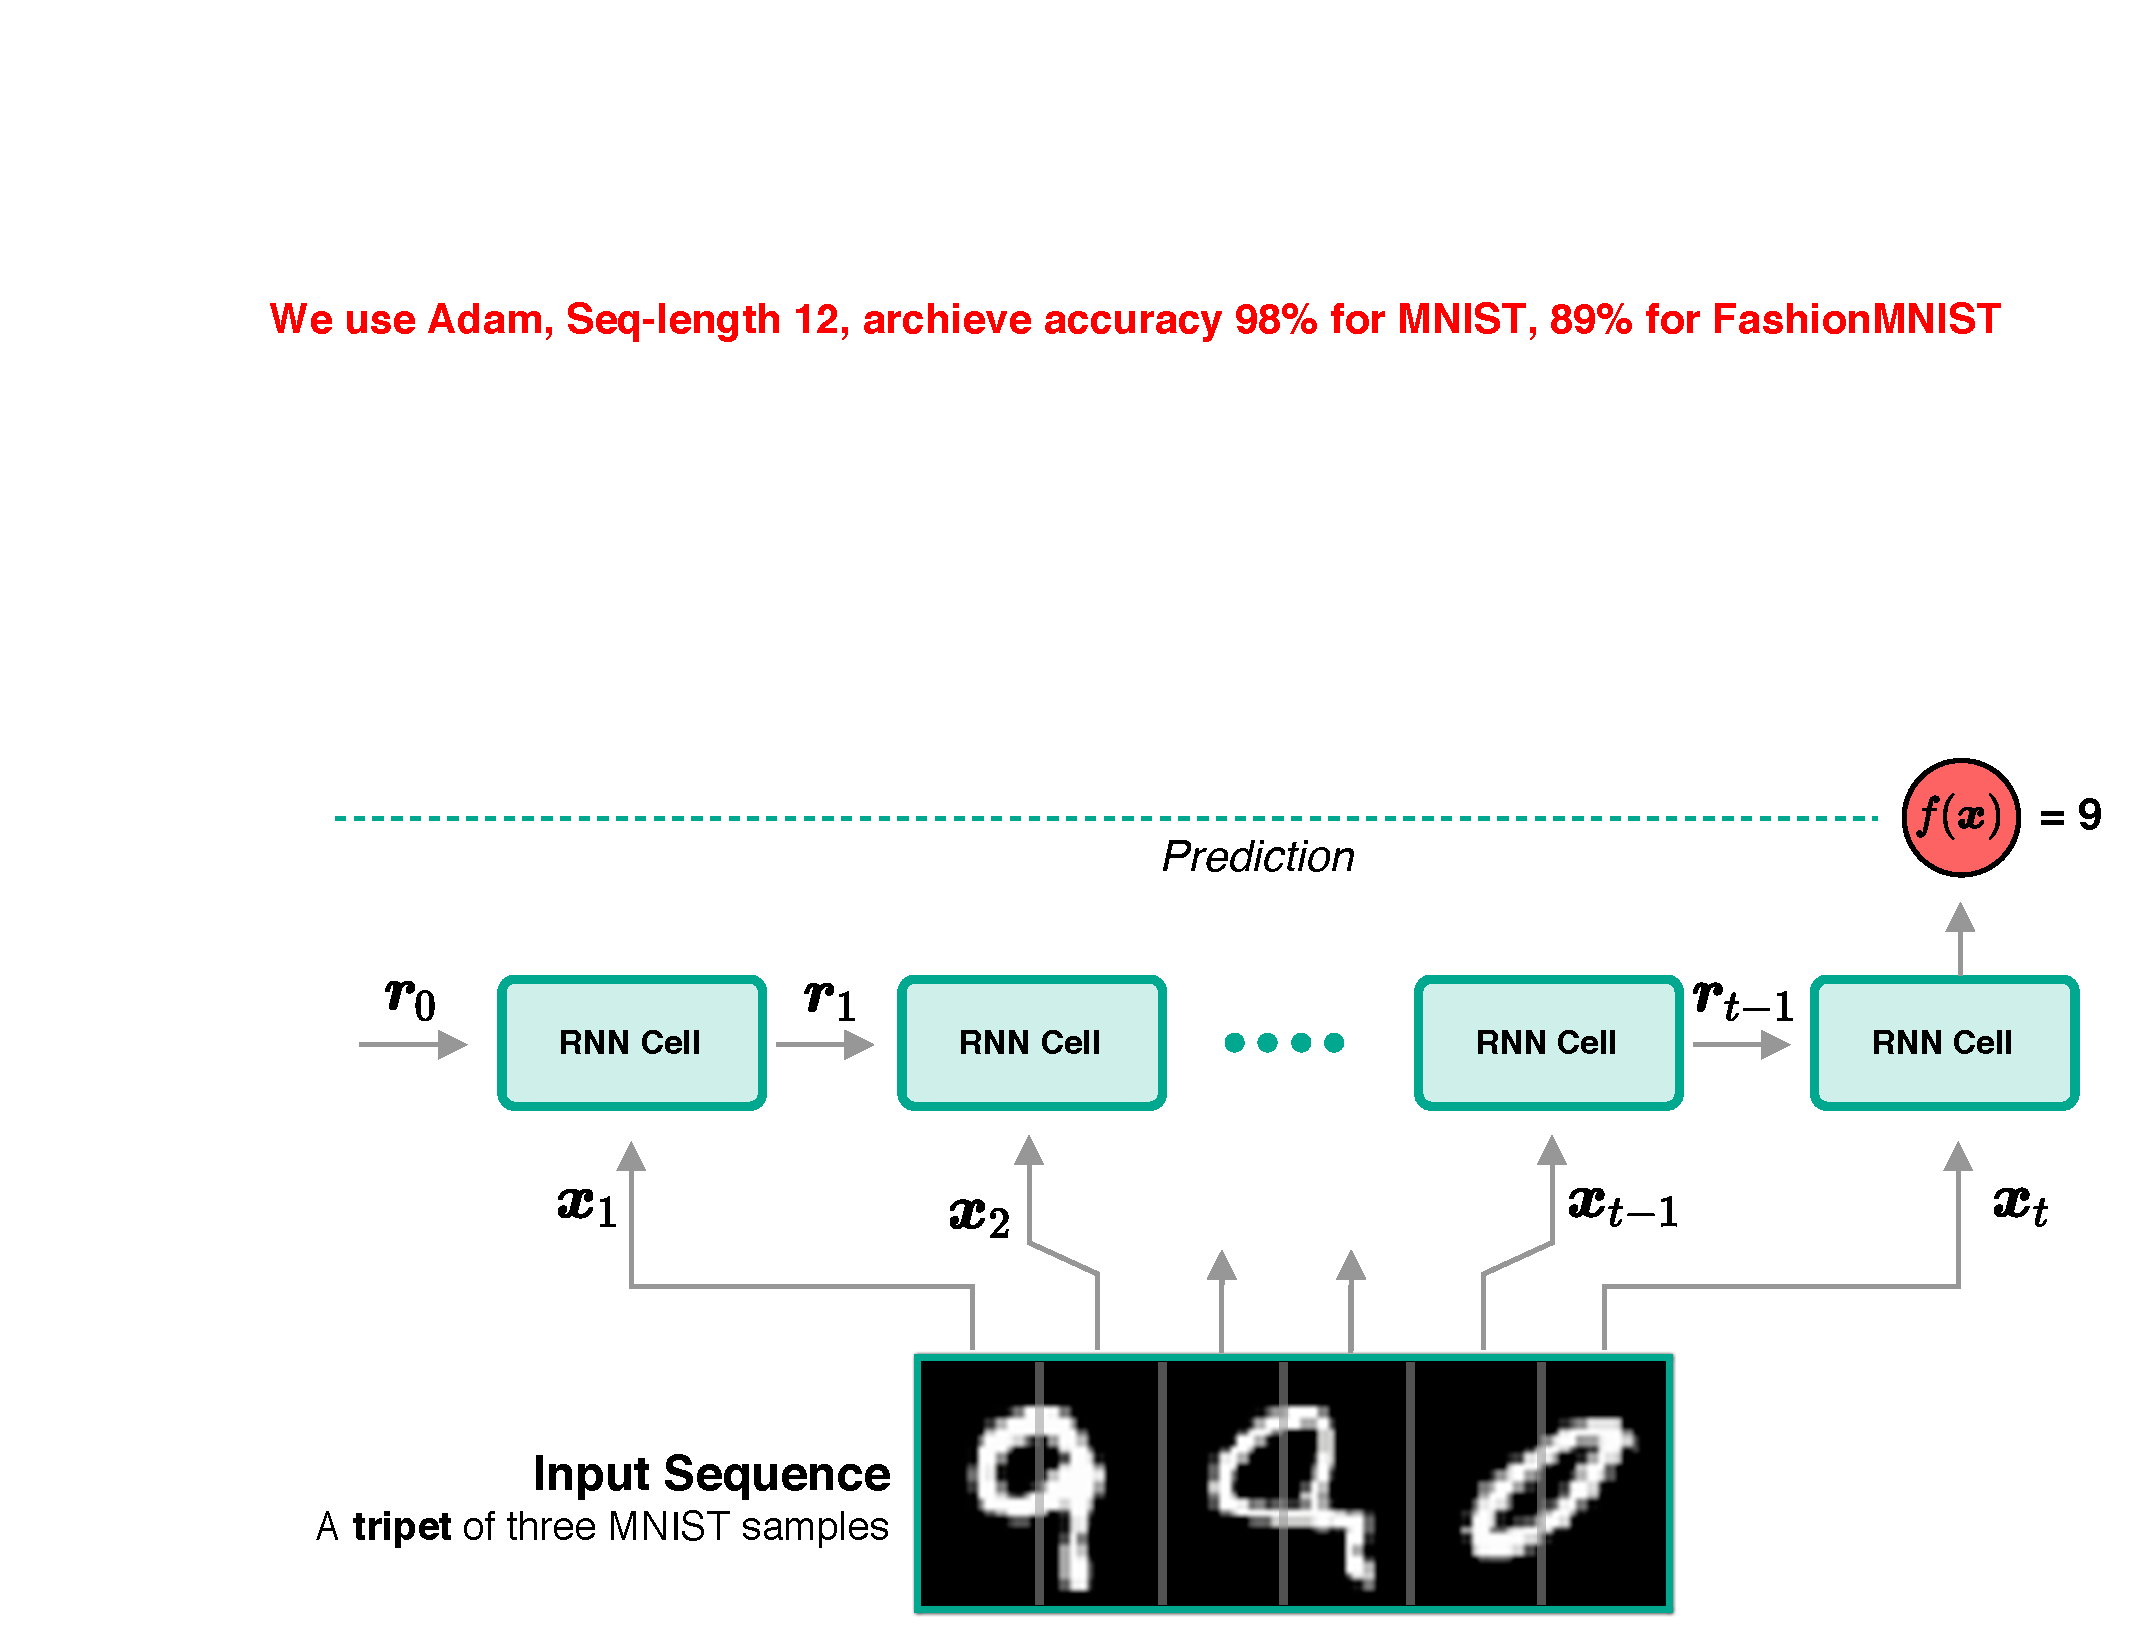
\includegraphics [width=0.65\textwidth]{figures/present_setting_1}
\end{figure}
}

\only<2>{
 \begin{figure}[h]
	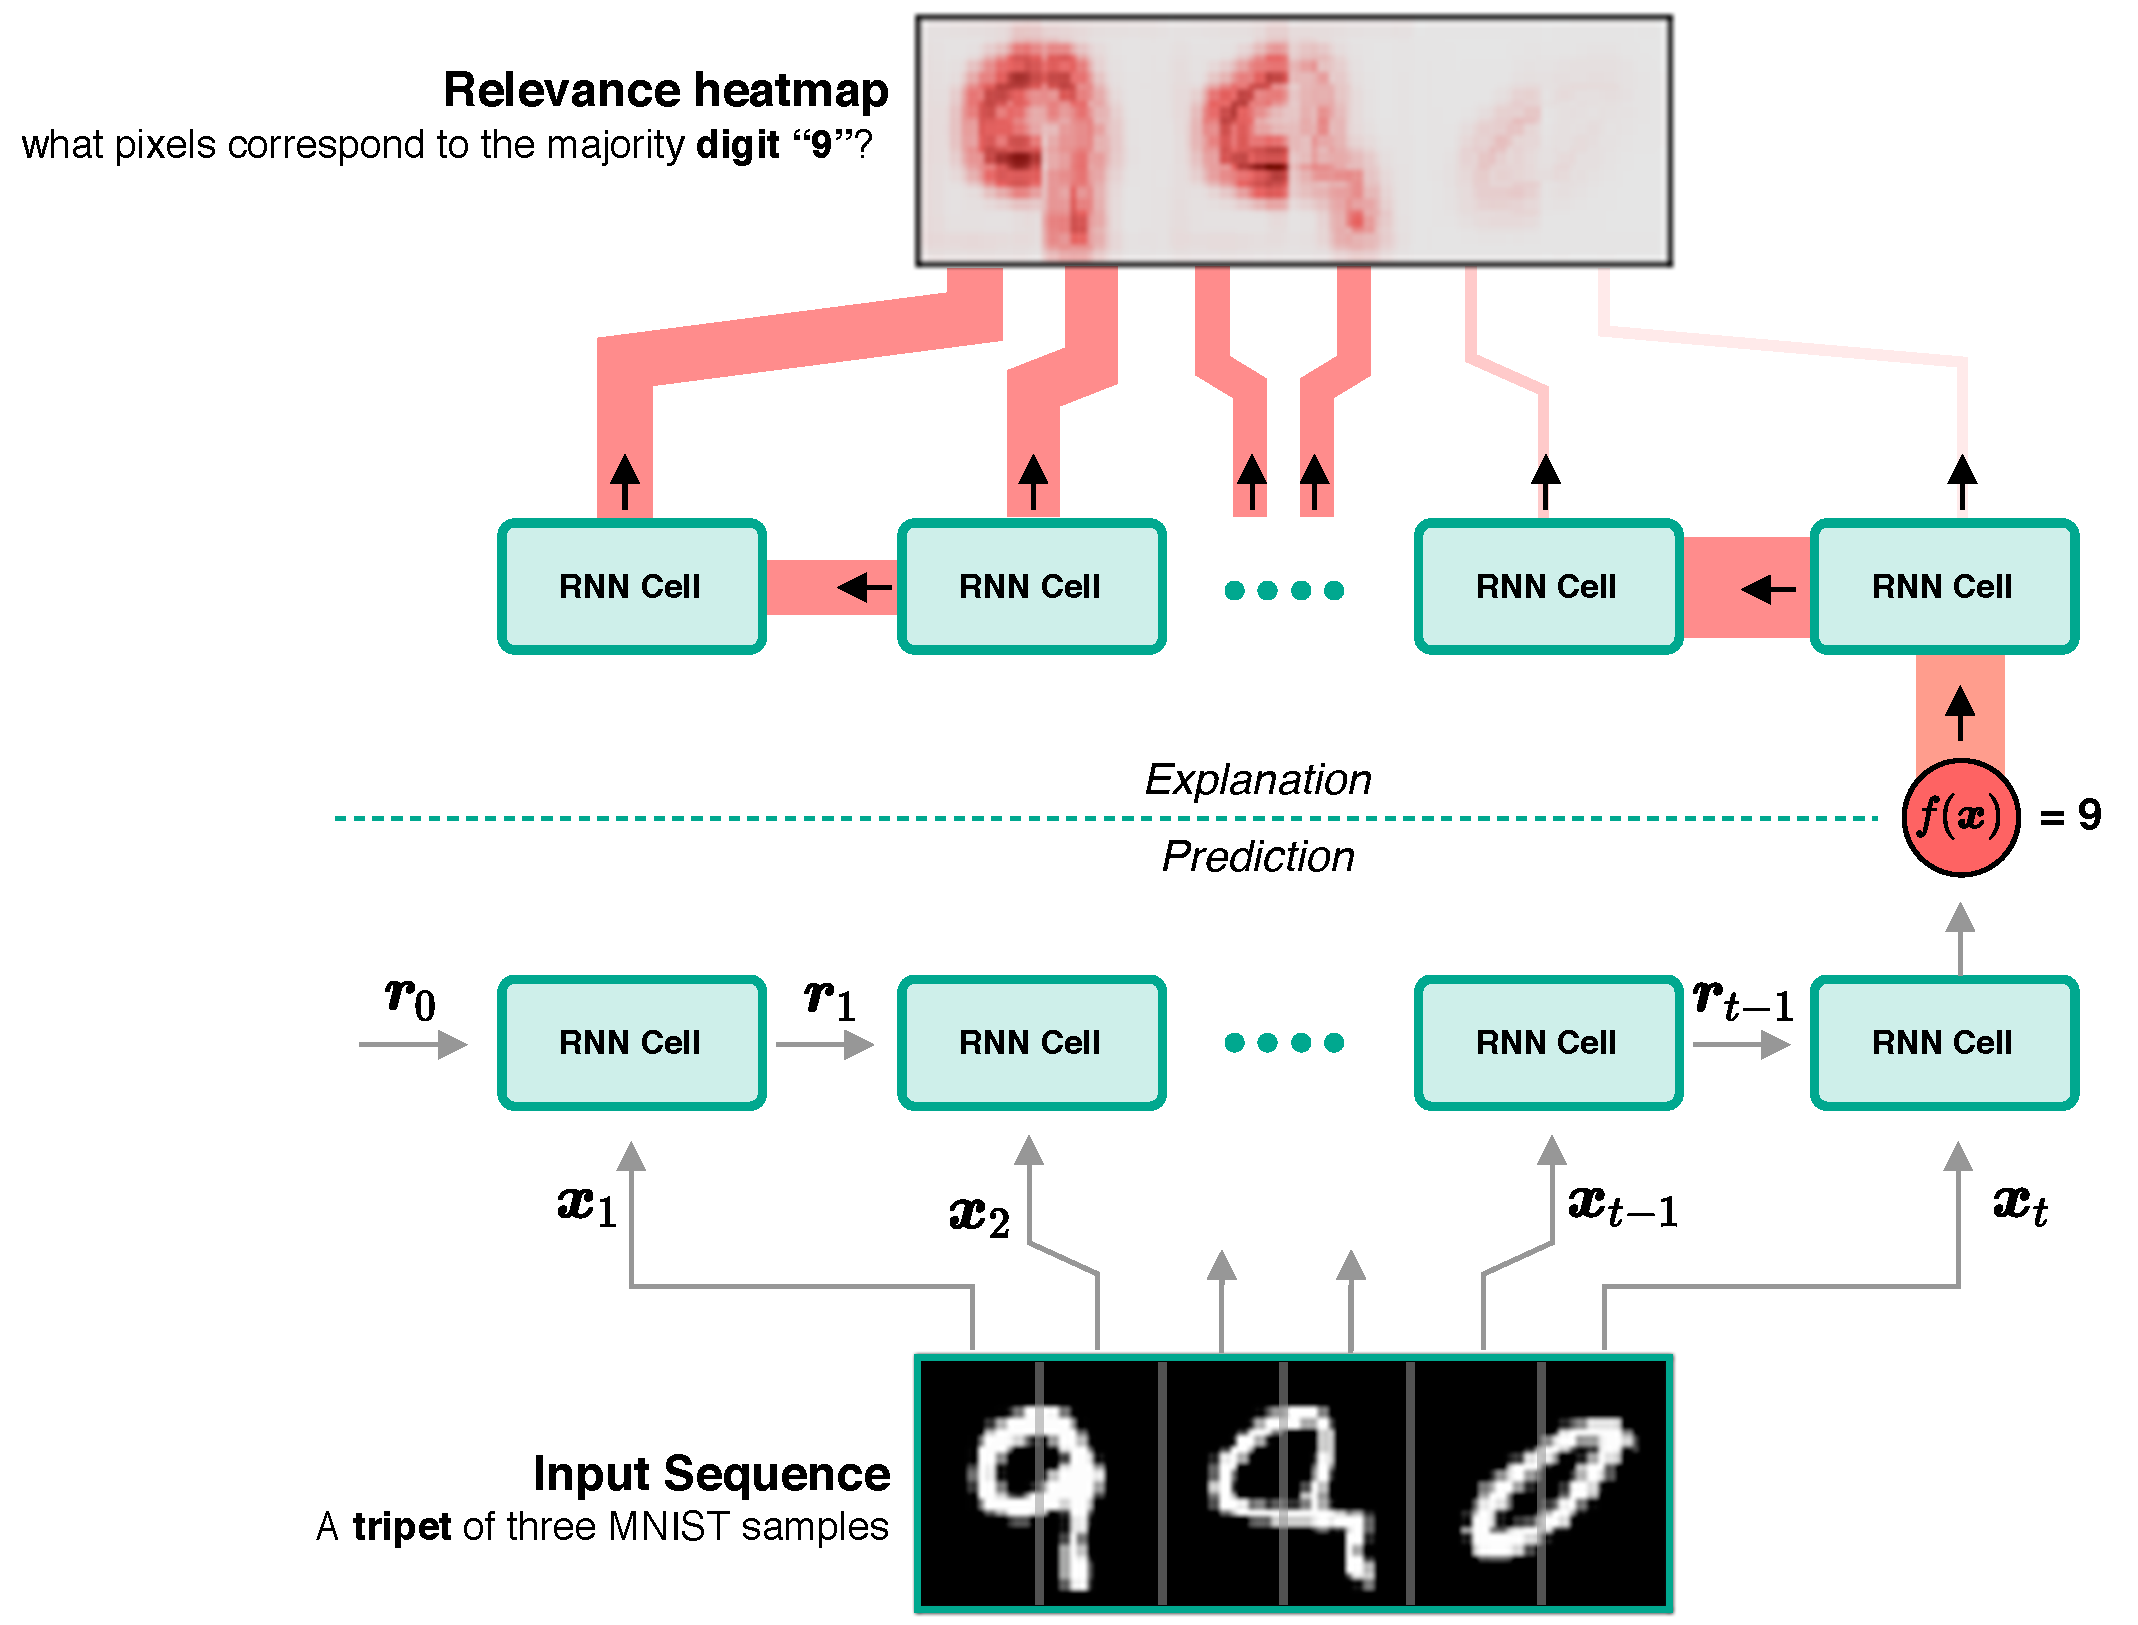
\includegraphics [width=0.65\textwidth]{figures/present_setting_2}
\end{figure}

}
	\item <3> \textbf{Evaluation:} Cosine similarity (averaged over test samples)
 \begin{figure}[h]
	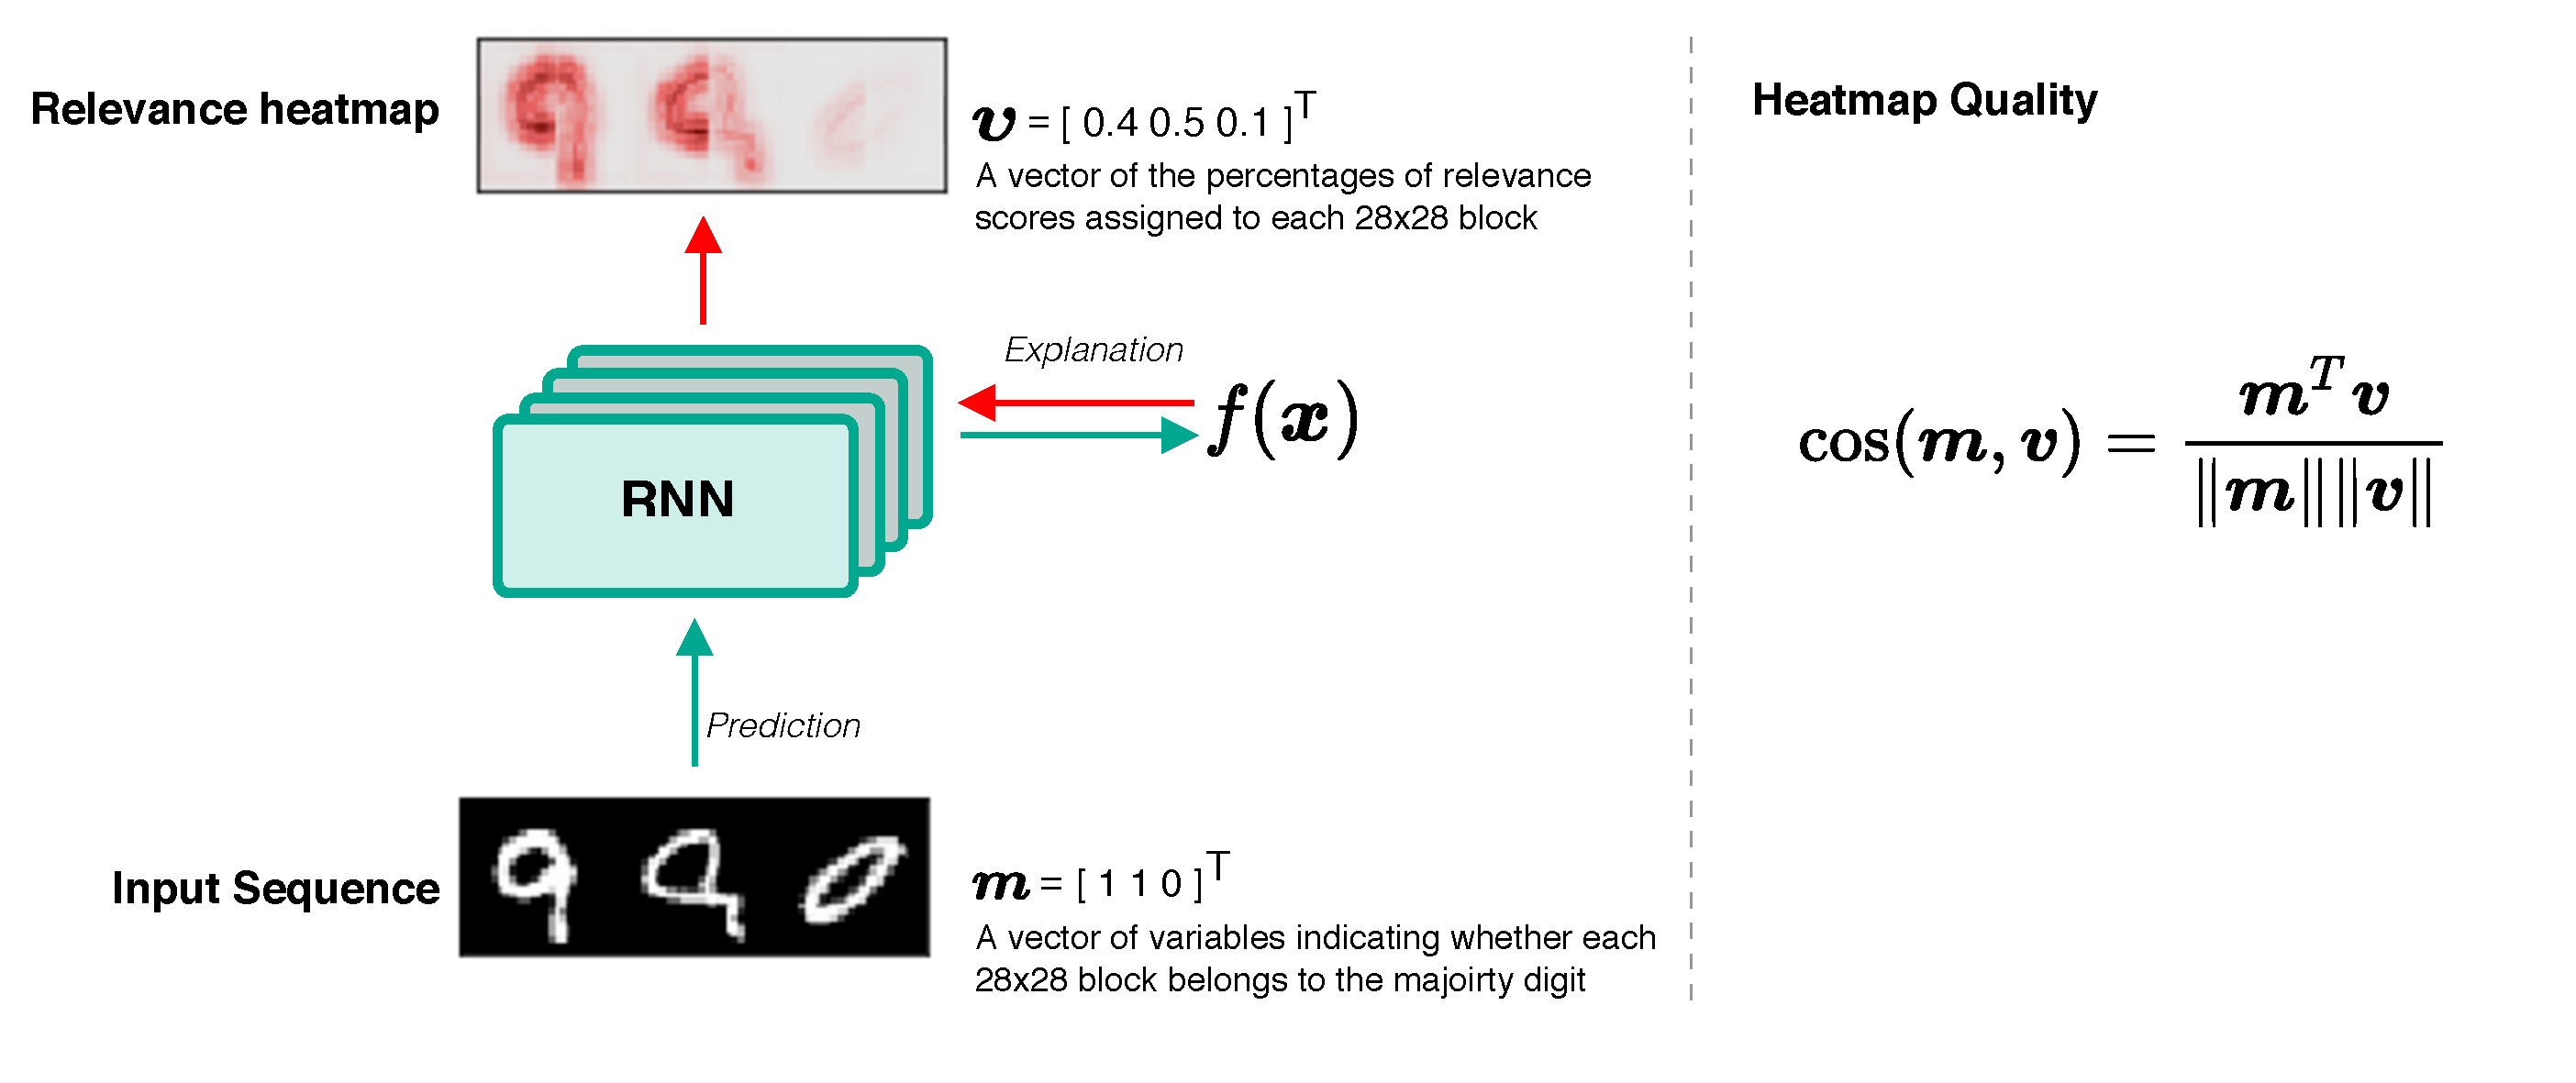
\includegraphics [width=0.85\textwidth]{figures/present_evaluation}
\end{figure}

\end{itemize}


\end{frame}

\begin{frame}{Experiment 1: Standard RNN Architectures}
\only<1>{

\vfill
 \begin{figure}[h]
	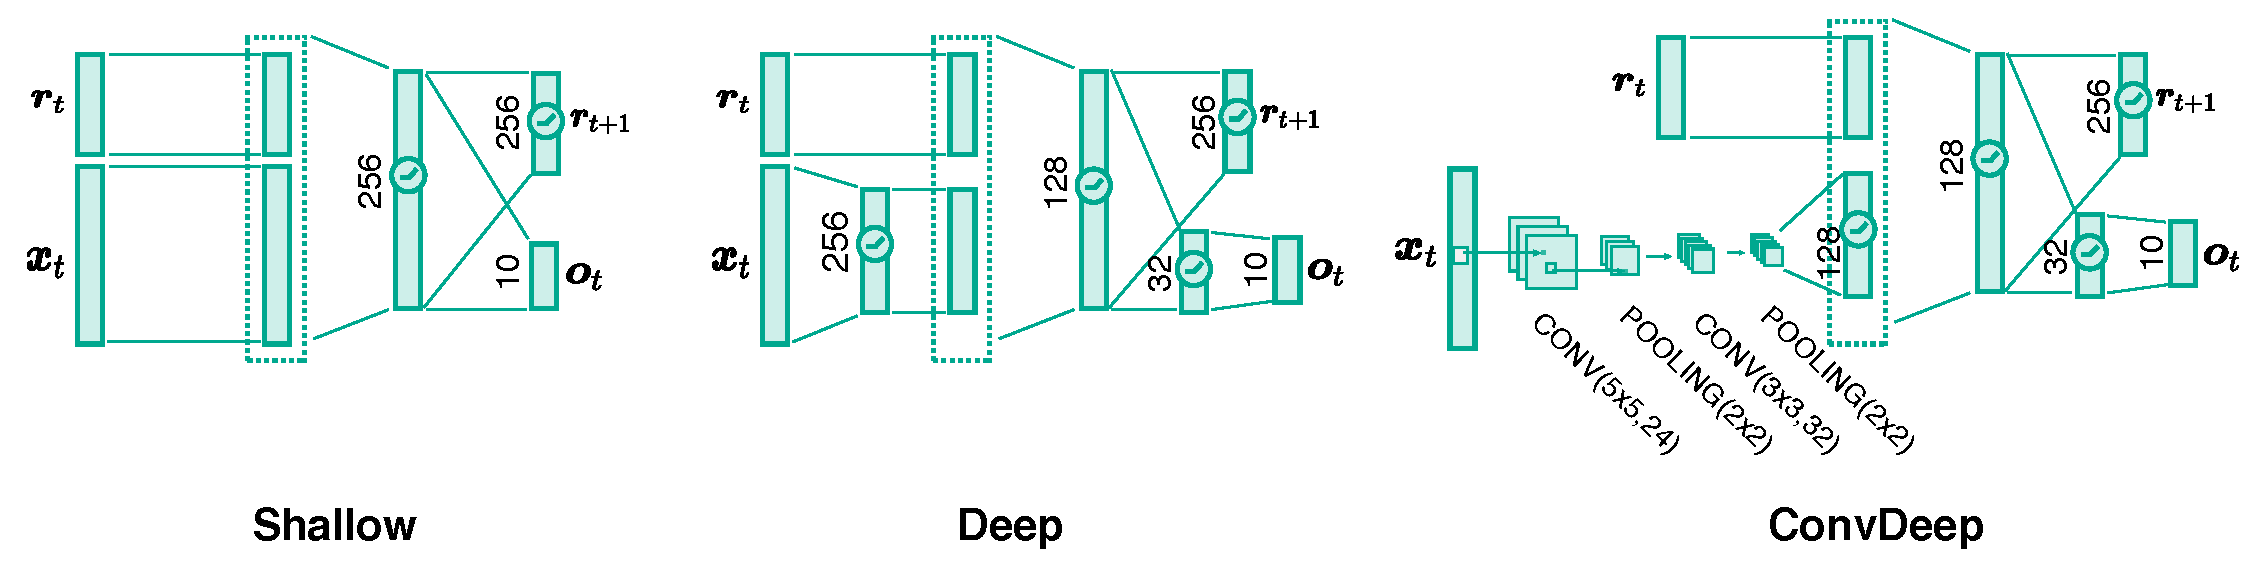
\includegraphics [width=\textwidth]{figures/present_exp1_standard_RNNs}
\end{figure}
\vfill
}
\only<2>{
Sample Relevance Heatmaps
\vfill
 \begin{figure}[h]
	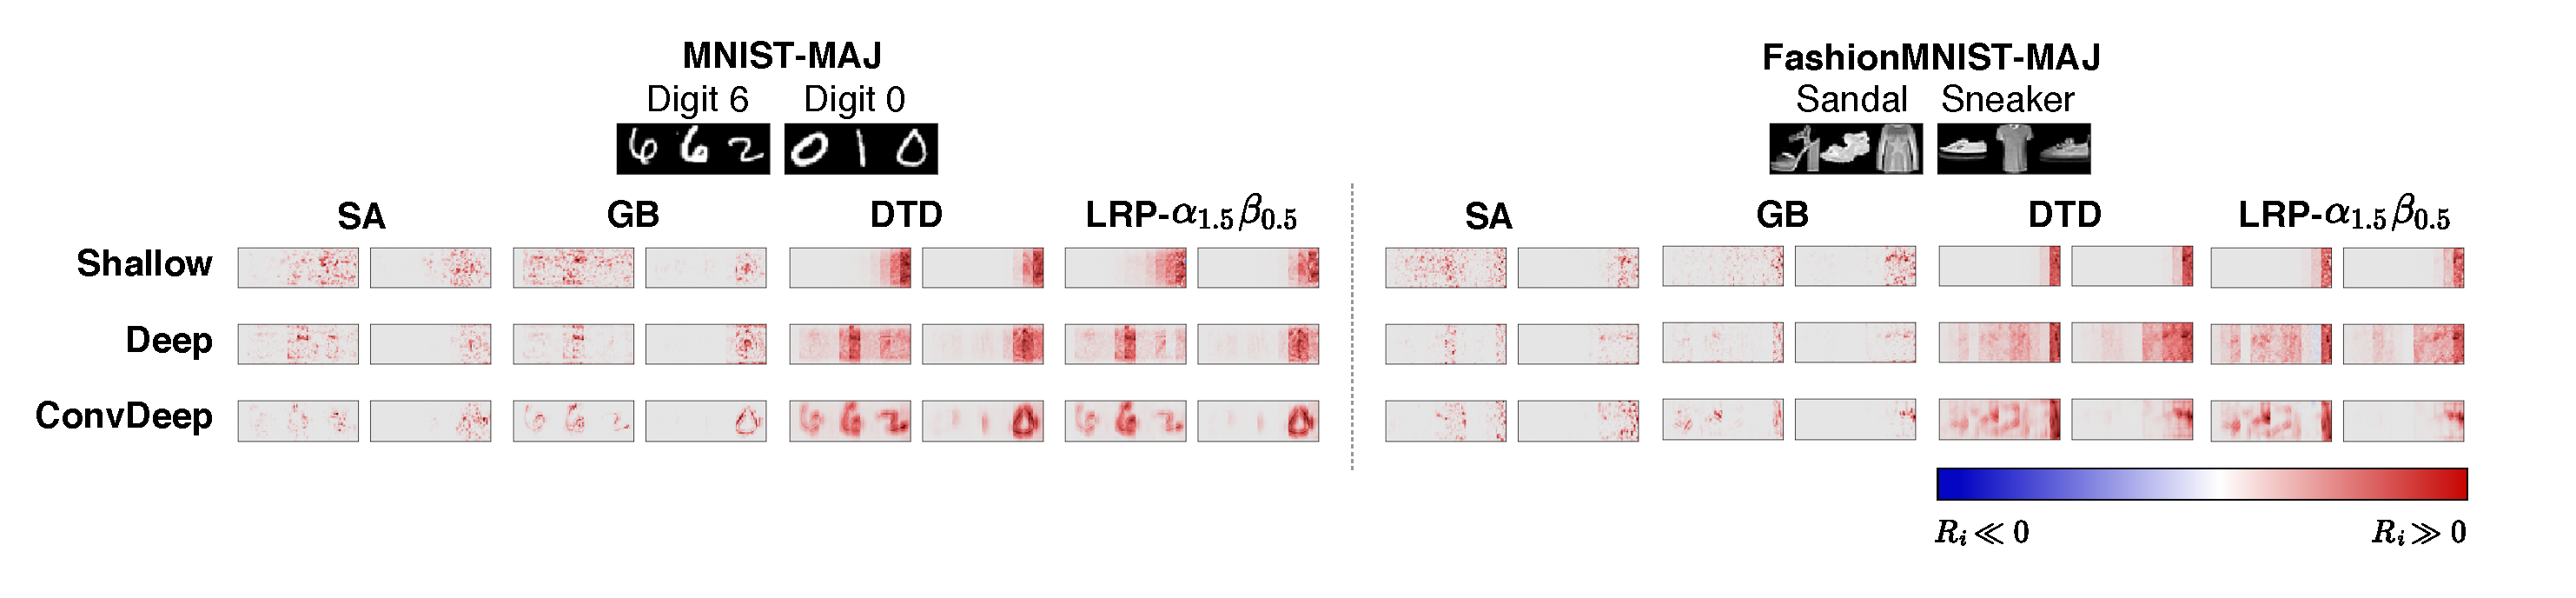
\includegraphics [width=\textwidth]{figures/present_exp1_result_heatmap}
\end{figure}
\vfill

}

\only<3>{
Cosine Similarity Evaluation
\vfill
 \begin{figure}[h]
	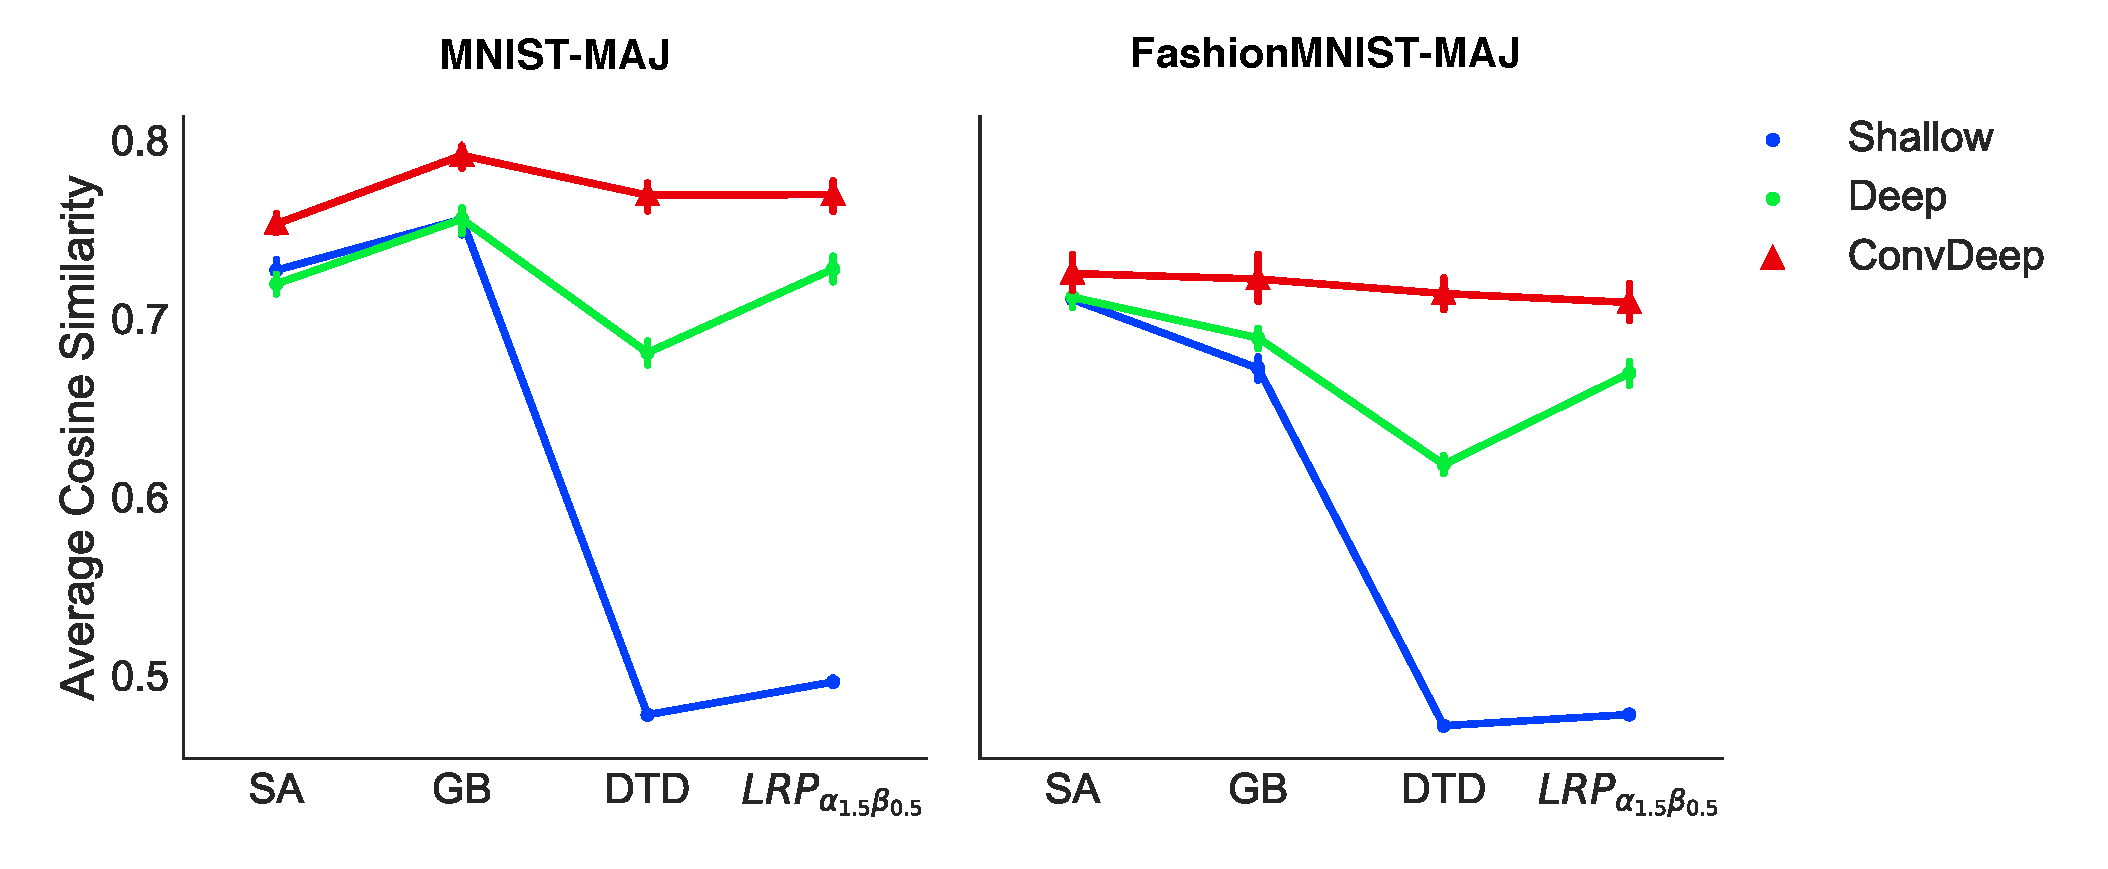
\includegraphics [width=\textwidth]{figures/present_exp1_result_eval}
\end{figure}
\vfill

}


\end{frame}
\begin{frame}{Experiment 2: More Explainable Models}

\only<1-3>{

\begin{enumerate}

	\item<1->LSTM \citep{HochreiterLongShortTermMemory1997} with tanh being replaced by ReLU (R-LSTM)

	\only<1>{
				--- Gating units are ignored during explaining \citep{ArrasExplainingRecurrentNeural2017}. 
		\vfill
		 \begin{figure}[h]
			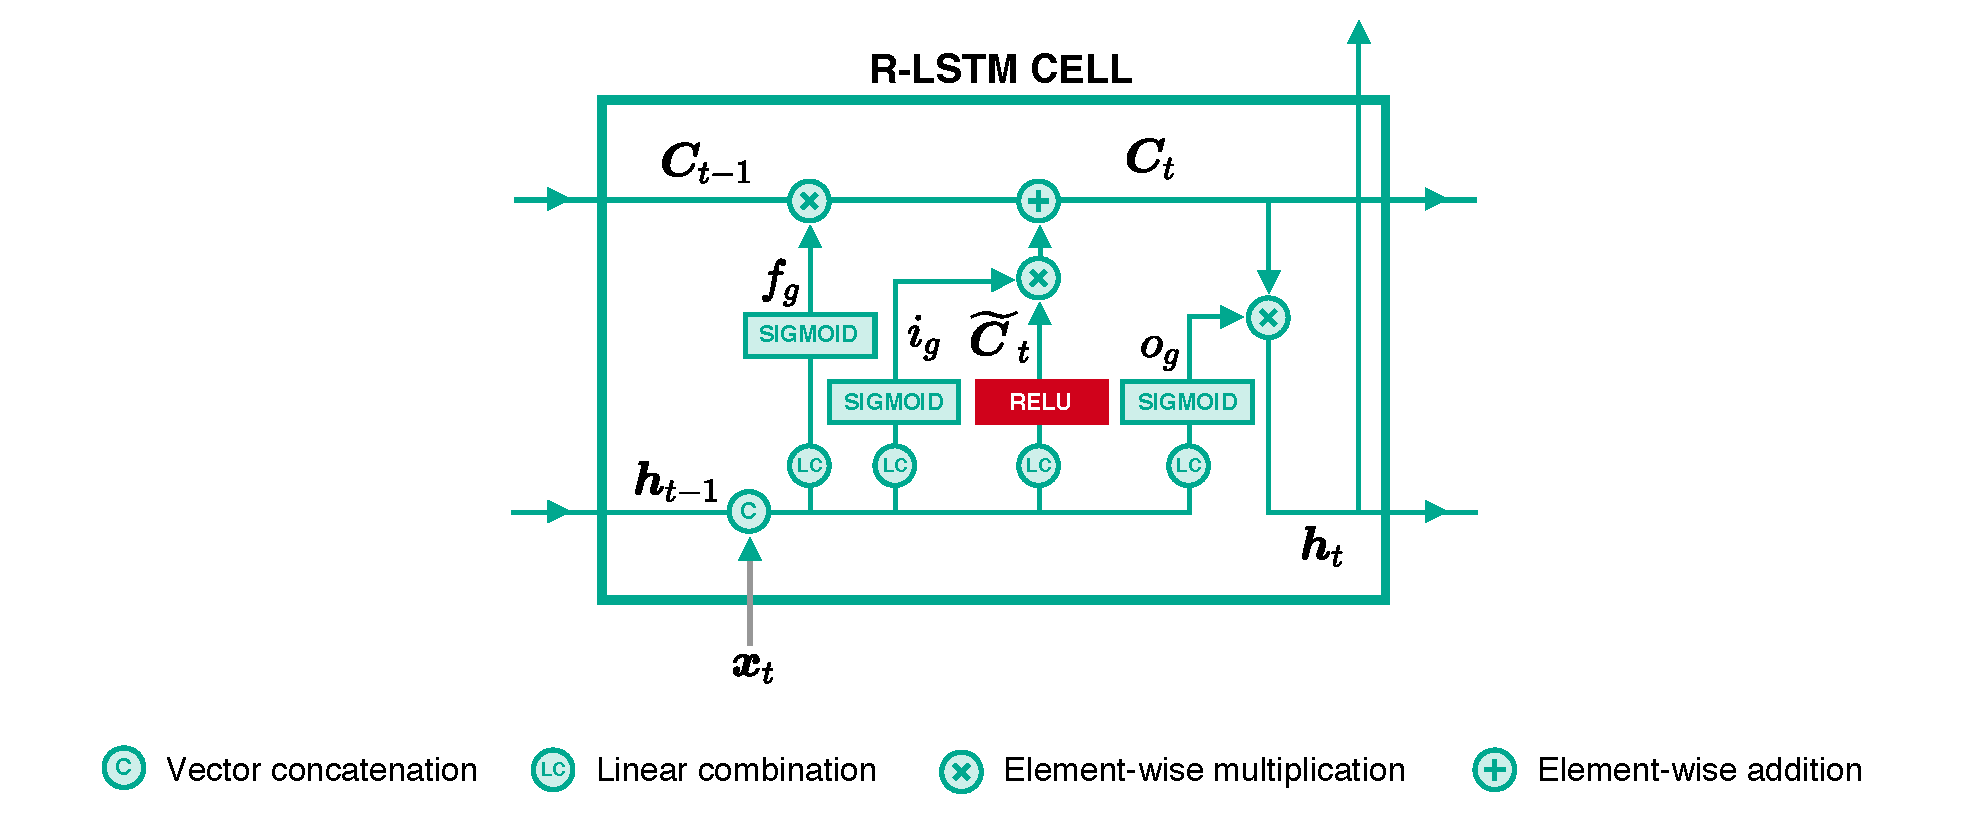
\includegraphics [width=\textwidth]{figures/present_rlstm}
		\end{figure}
		\vfill

	}
	\item<2-> 
	Stationary Dropout 
		\citep{GalTheoreticallyGroundedApplication2016}  (-SD)
		\only<2>{
		\vfill
		 \begin{figure}[h]
			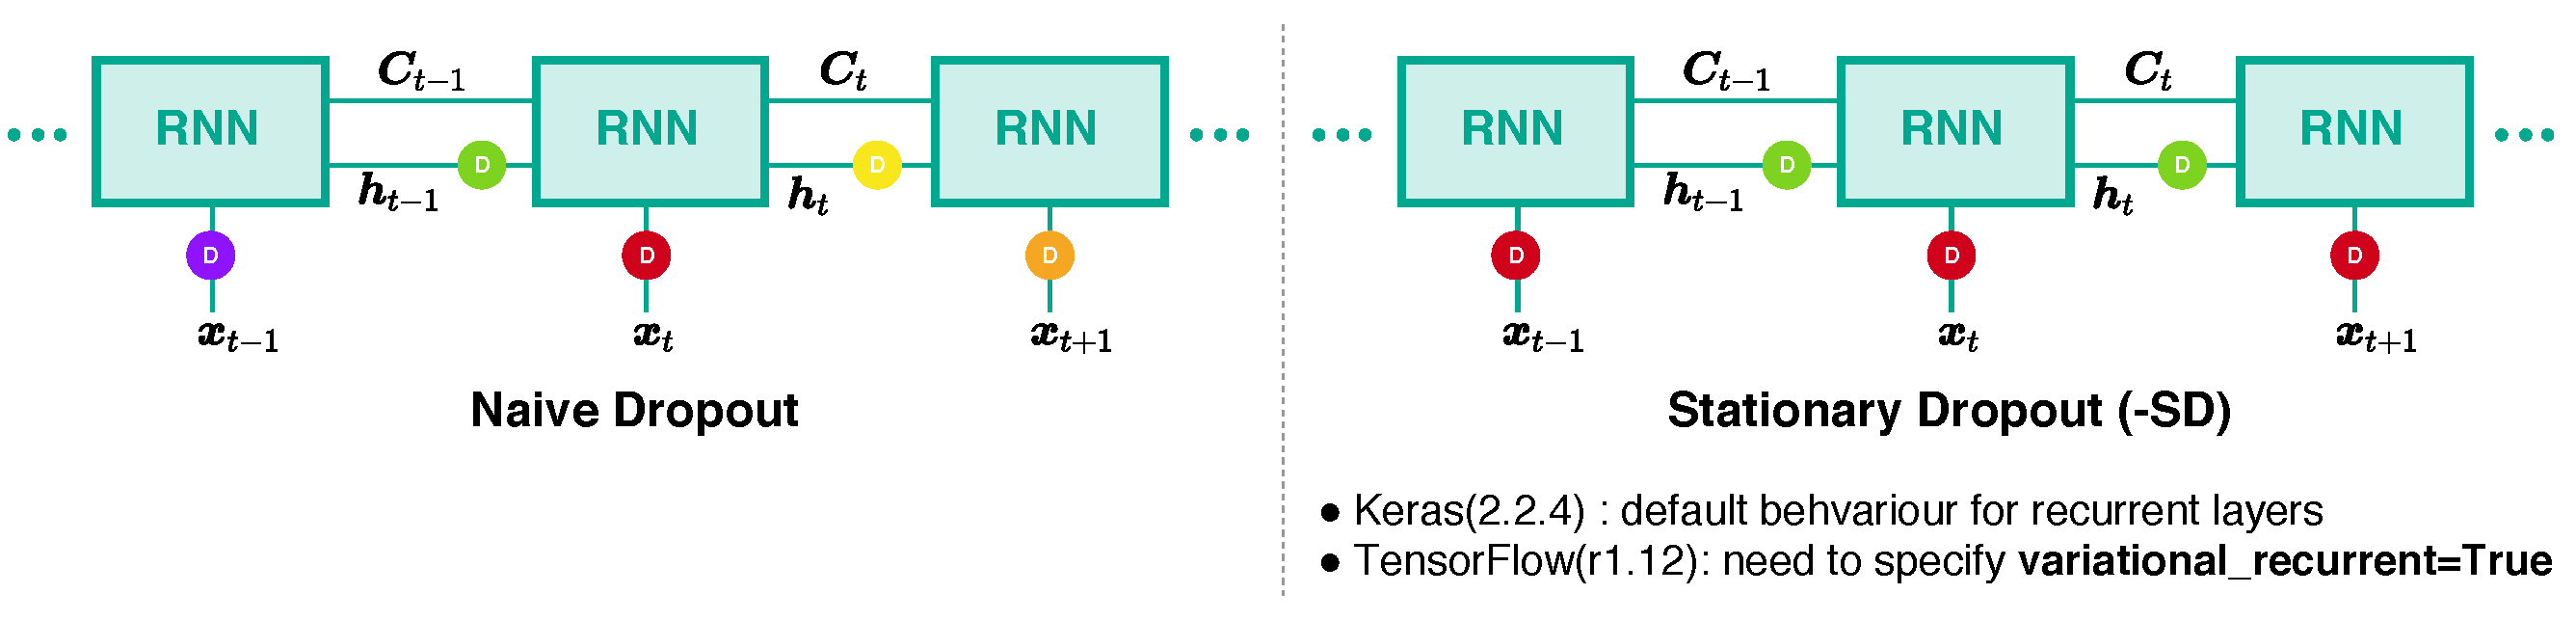
\includegraphics [width=0.9\textwidth]{figures/present_dropout_comparison}
		\end{figure}
		\vfill
		}
		
	\item<3> { Lateral Connections for convolutional layers (Conv$^+$)
		\only<3>{
			\vfill
		 \begin{figure}[h]
			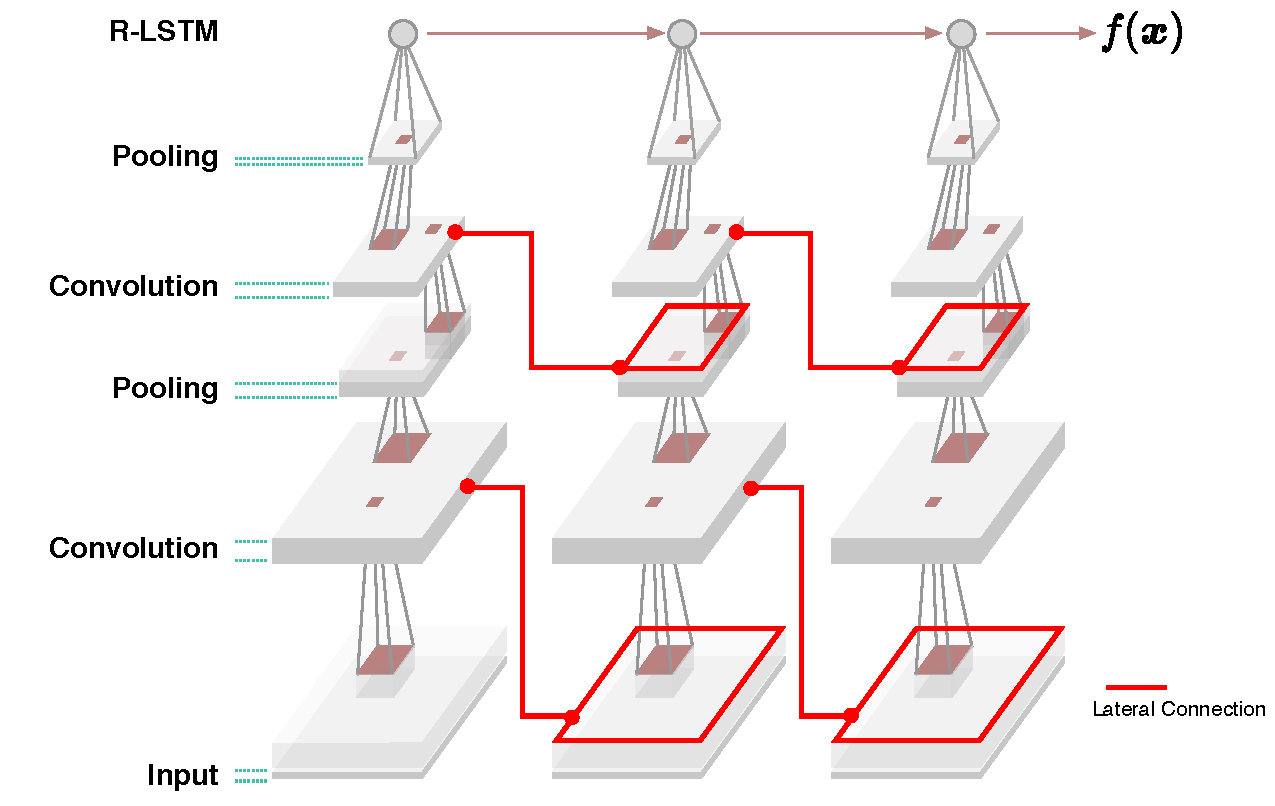
\includegraphics [width=0.6\textwidth]{figures/present_conv_lat_rlstm}
		\end{figure}
		\vfill
		}
		
	}
\end{enumerate}
}

		\only<4>{
		Sample Relevance Heatmaps
		\vfill
		
		 \begin{figure}[h]
			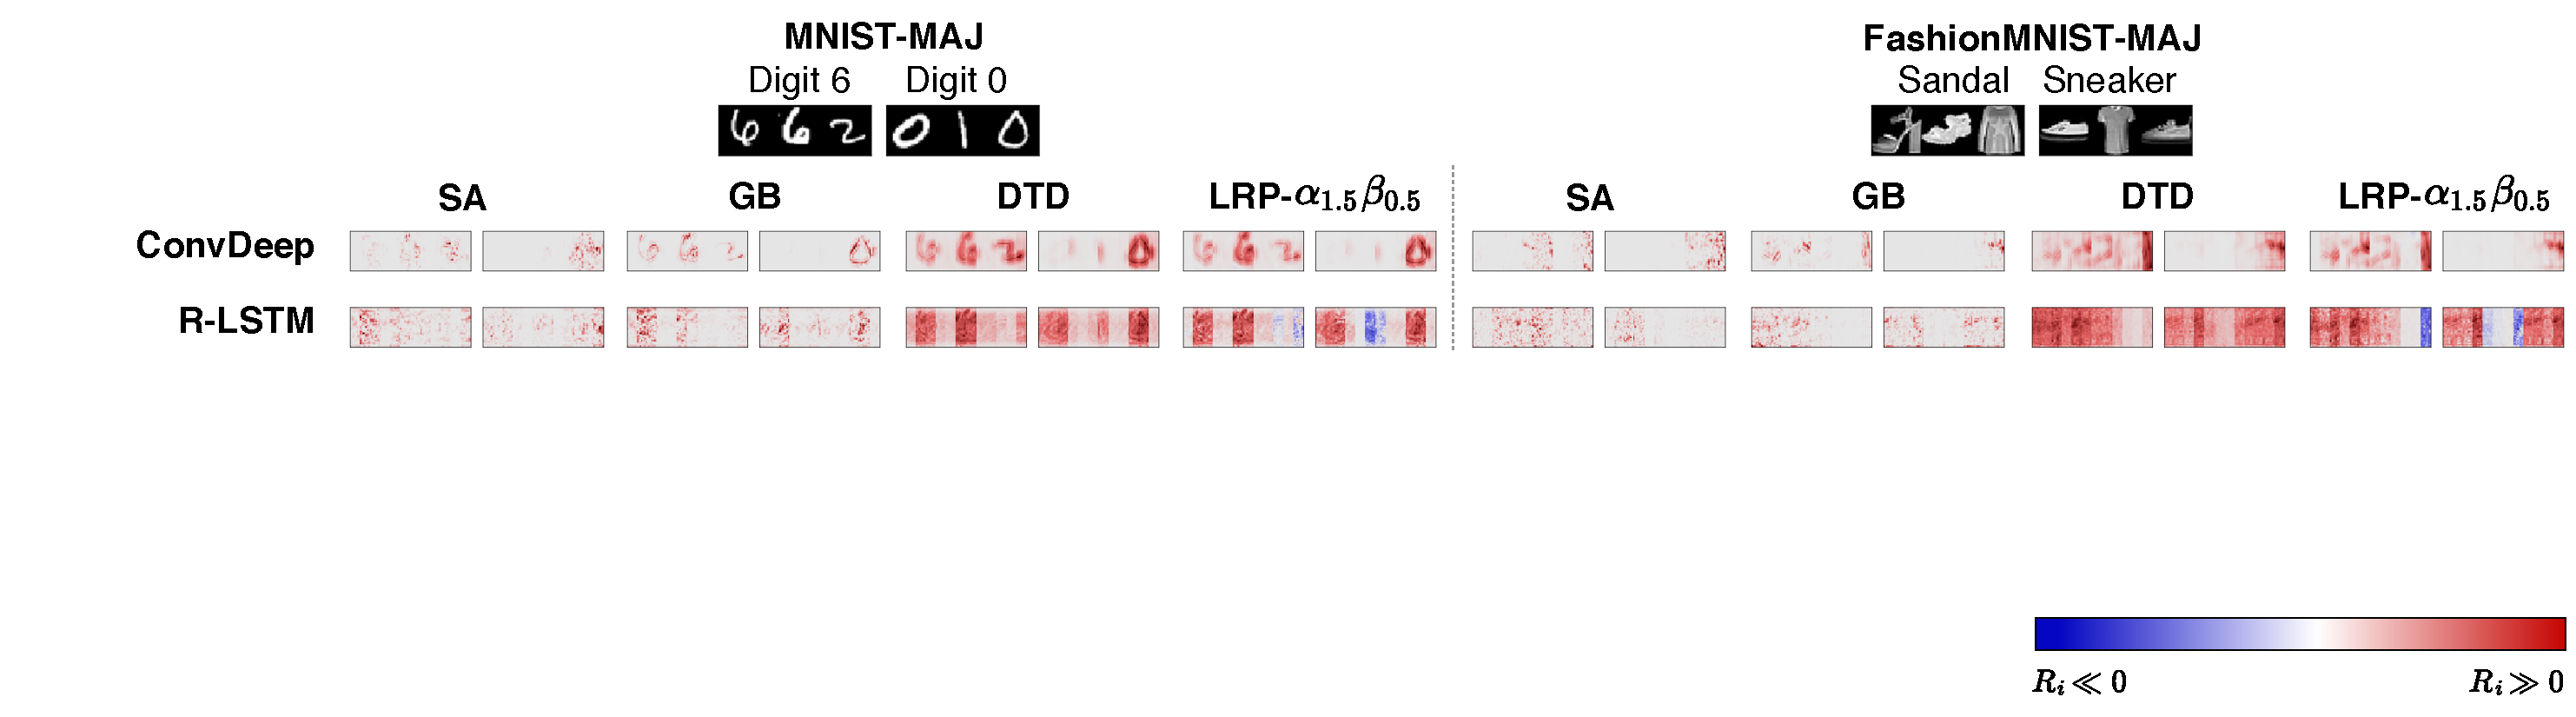
\includegraphics [width=\textwidth]{figures/present_exp2_result_heatmap_1}
		\end{figure}
		
		\vfill
		
		}
		\only<5>{
		Sample Relevance Heatmaps
		\vfill
		
		 \begin{figure}[h]
			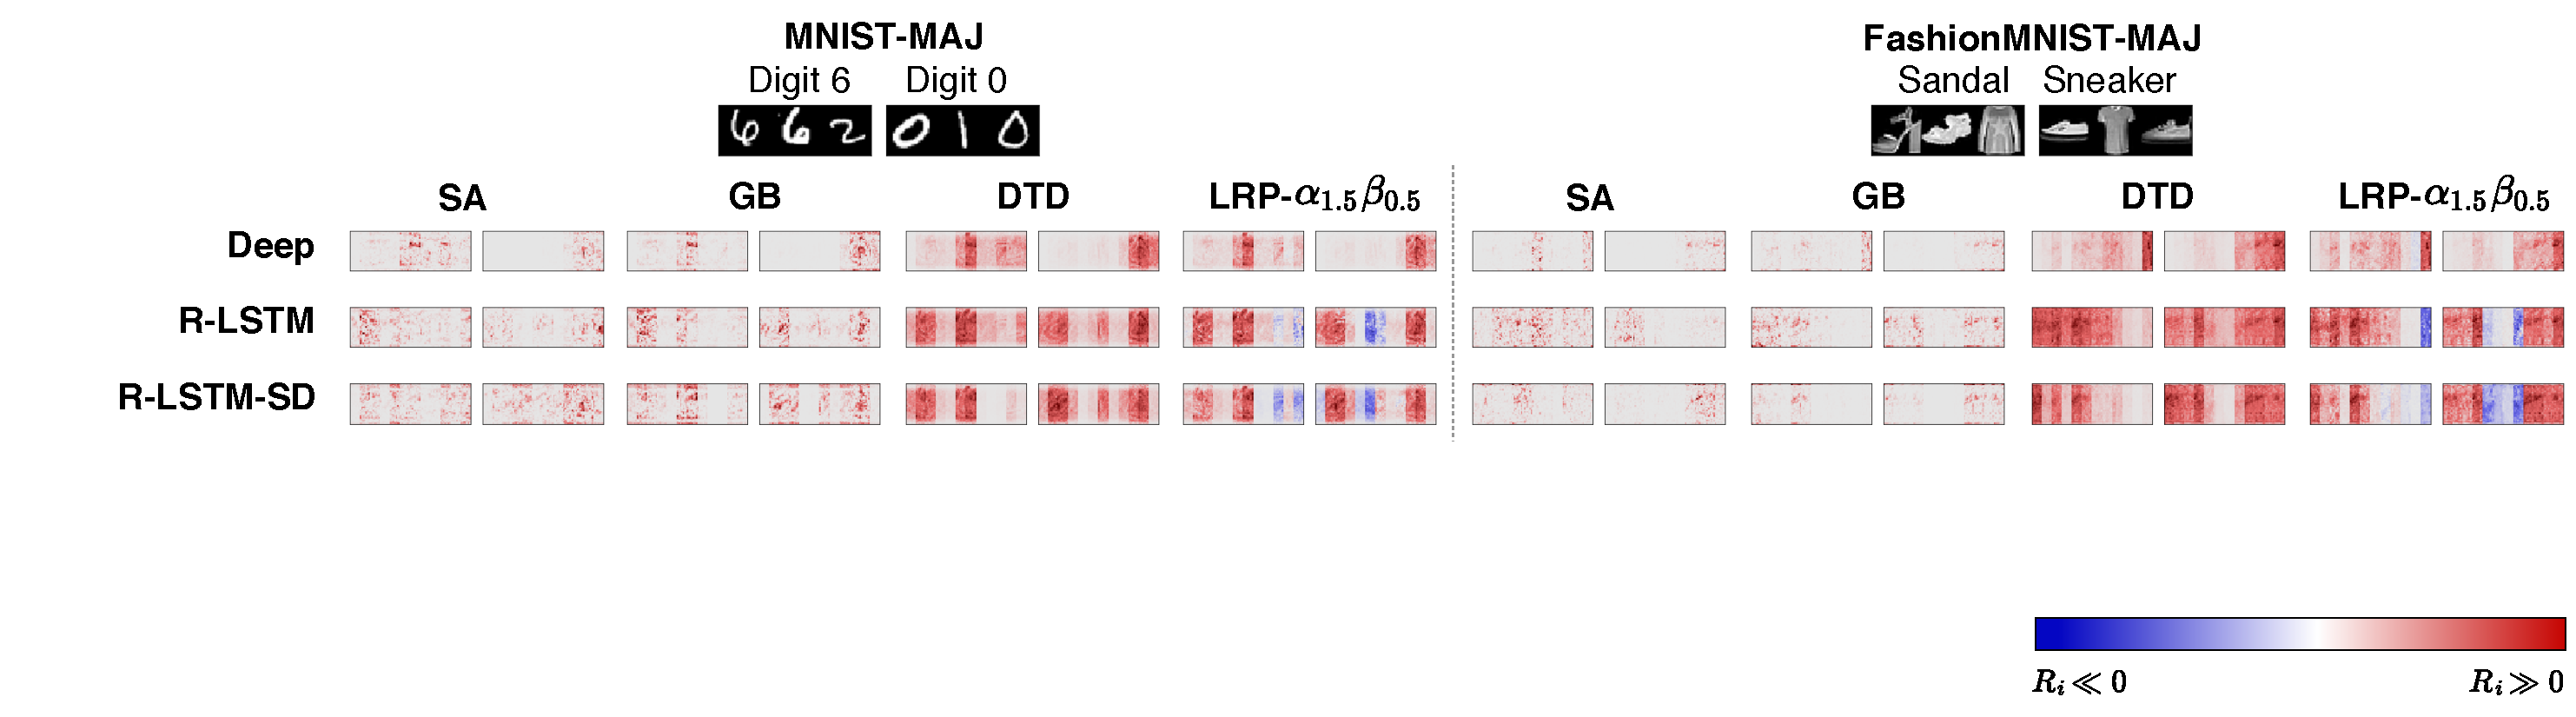
\includegraphics [width=\textwidth]{figures/present_exp2_result_heatmap_2}
		\end{figure}
		
		\vfill
		
		}
		
		\only<6>{
Cosine Similarity Evaluation
\vfill
 \begin{figure}[h]
	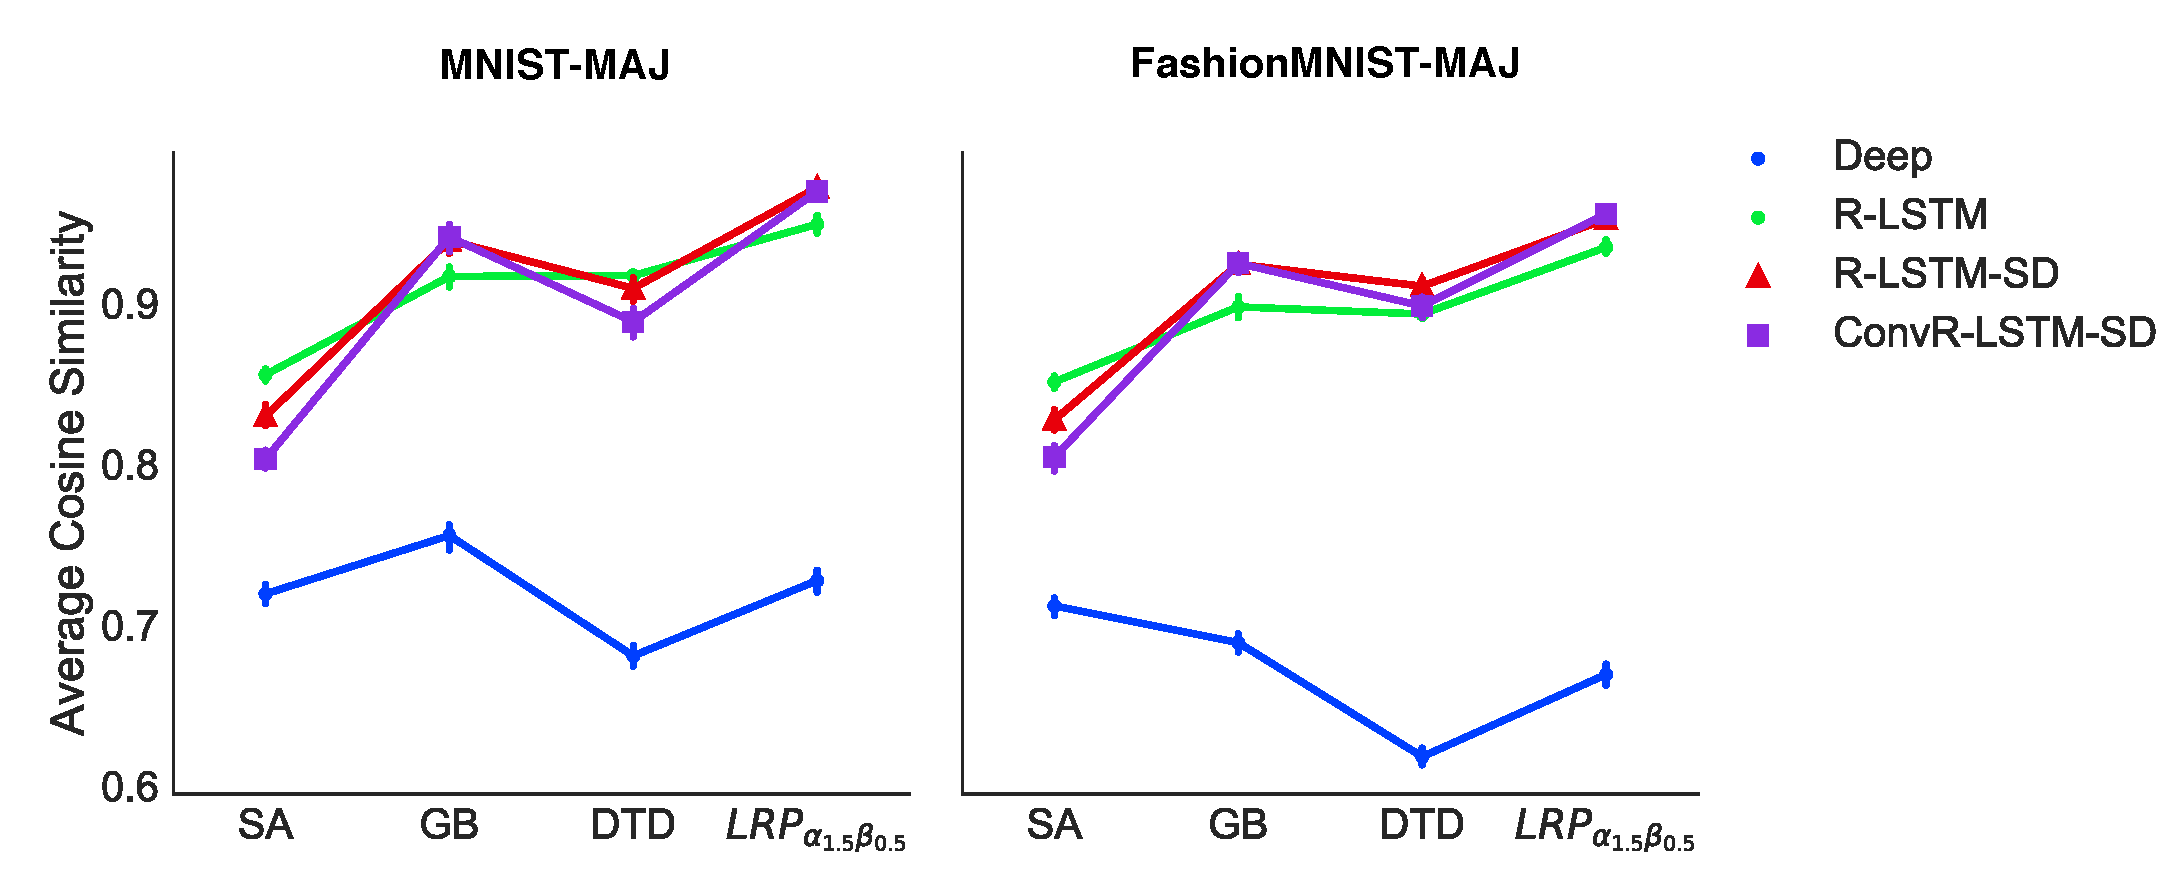
\includegraphics [width=\textwidth]{figures/present_exp2_result_eval}
\end{figure}
\vfill

}
		
		\only<7>{
		Sample Relevance Heatmaps
		\vfill
		
		 \begin{figure}[h]
			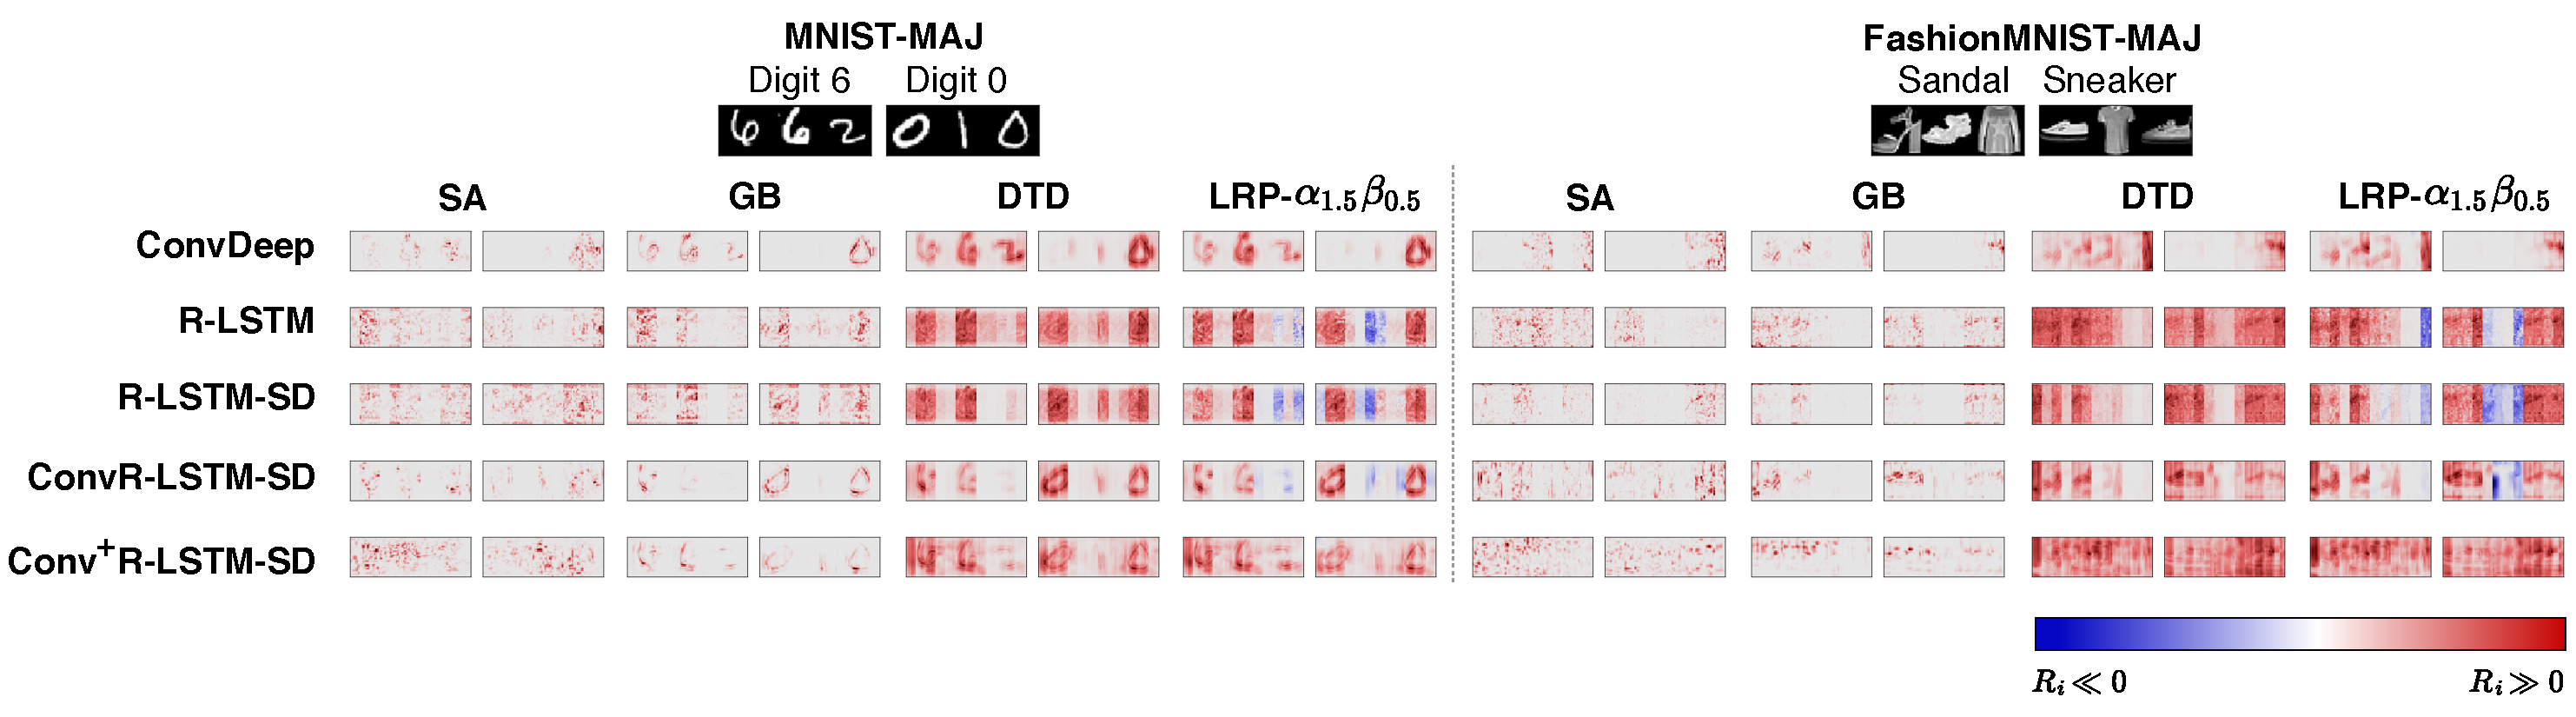
\includegraphics [width=\textwidth]{figures/present_exp2_result_heatmap_3}
		\end{figure}
		
		\vfill
		
		}


\only<8>{
Cosine Similarity Evaluation
\vfill
 \begin{figure}[h]
	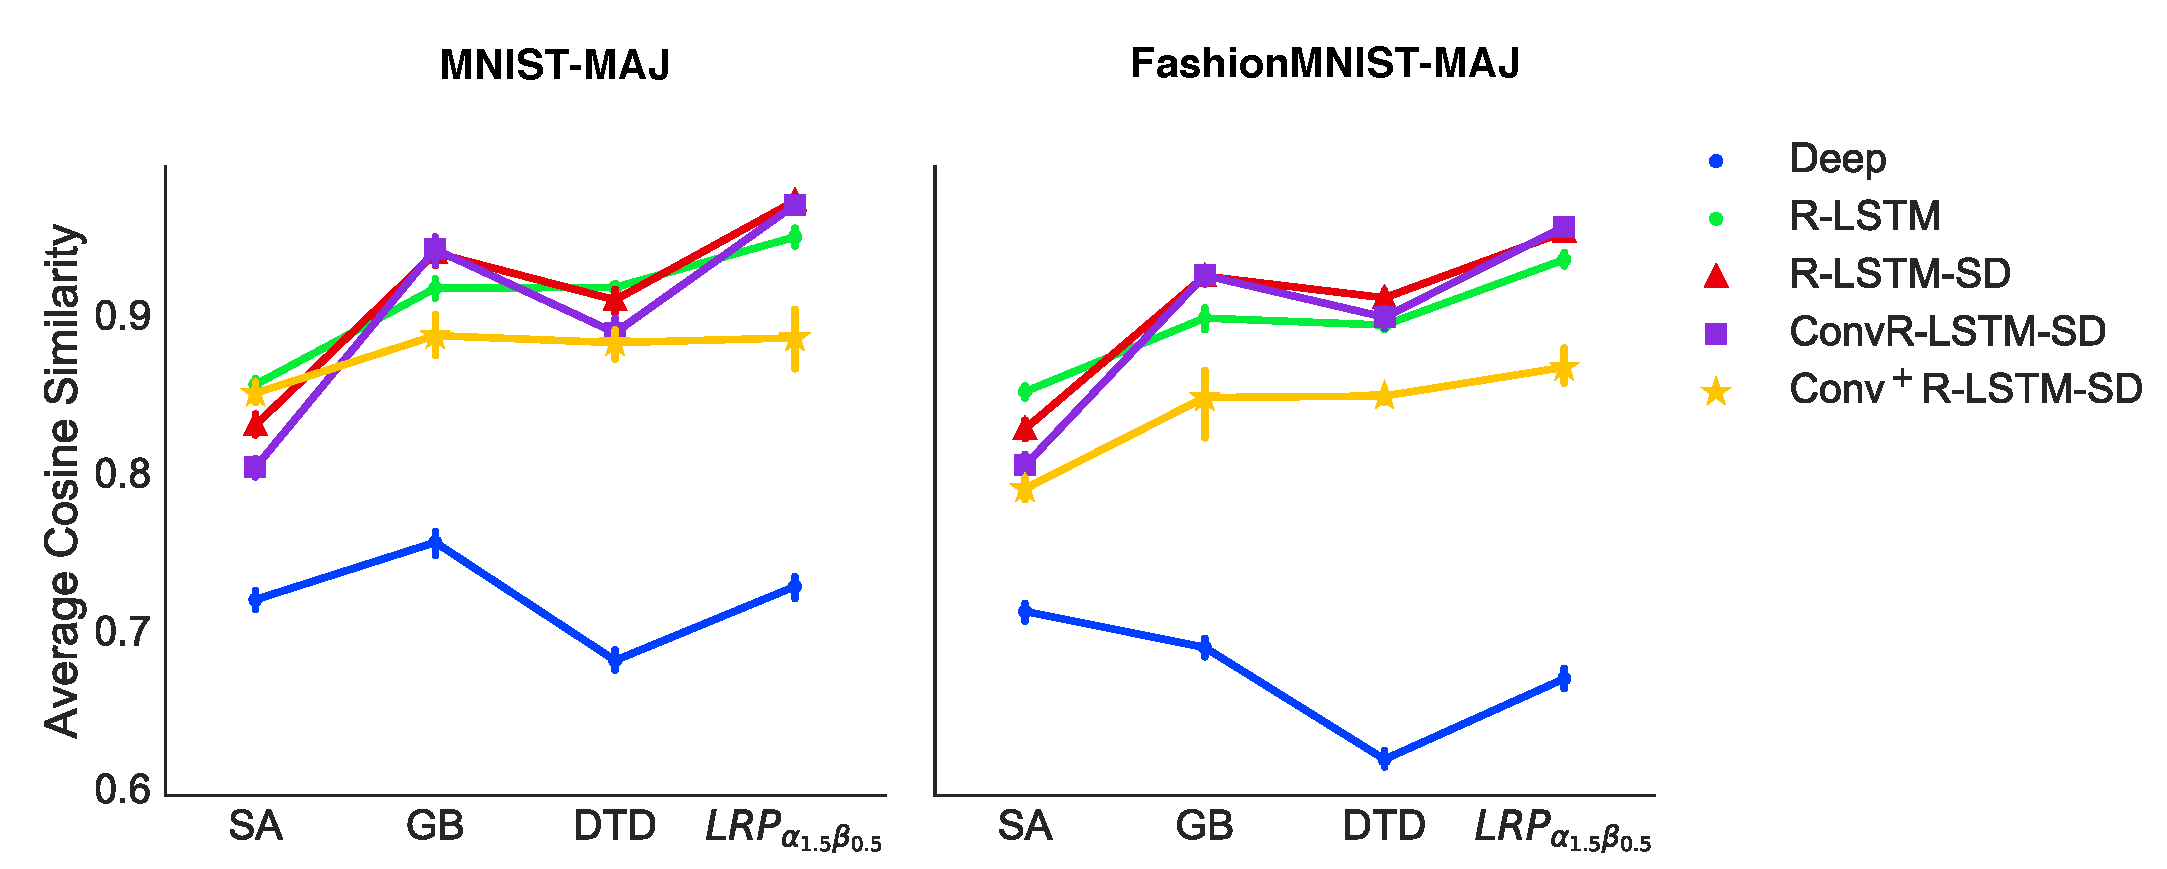
\includegraphics [width=\textwidth]{figures/present_exp2_result_eval_2}
\end{figure}
\vfill

}


\end{frame}


\begin{frame}{Conclusion}

\begin{itemize}
	\item \textbf{Deeper and LSTM-type RNNs} have more explainable predictions.
	\item \textbf{Stationary dropout} could improve model's explainability.
	\item Explainability of RNNs should be considered in two aspects:
		\begin{itemize}
			\item \textbf{Coarse-gained}: relevance adequately propagated to the relevant input steps \\
					--- related to recurrent mechanism (solution: LSTMs)
			\item \textbf{Fine-gained}: soundness of each input's explanation.\\
					--- related to the choice of input layers (i.e. convolutional layer for image data)
		\end{itemize}
	\item Part of this work will appear in: \\
{ \small \vspace{0.2cm}
Rieger, L., Chormai, P., Montavon, G., Hansen, L. K., \& Müller, K.-R. (2018). \textbf{Structuring Neural Networks for More Explainable Predictions.} In H. Jair Escalante, S. Escalera, I. Guyon, X. Baró, Y. Güçlütürk, U. Güçlü, \& M. A. J. van Gerven (Eds.), Explainable and Interpretable Models in Computer Vision and Machine Learning (1st ed., p. 299). Springer International Publishing.

}

\end{itemize}
\end{frame}


\begin{frame}{}
\vfill \centering
\LARGE \textbf{Q\&A}
\vfill
\end{frame}

\begin{frame}[allowframebreaks]
        \frametitle{References}
        \bibliographystyle{amsalpha}
        \bibliography{references.bib}
\end{frame}
\end{document}
